\documentclass[twoside]{article}
\usepackage{../estilo-ejercicios}
\usepackage{wasysym}
\usetikzlibrary{automata,positioning}
\usepackage{mathdots}
\usepackage{listings}
%--------------------------------------------------------
\begin{document}

\title{Ciencias de la Computación}

\author{Javier Aguilar Martín}
\maketitle

\begin{ejercicio}{1}
Para cada uno de los siguientes lenguajes sobre el alfabeto $\Sigma=\{a,b\}$, construye un autómata finito determinista que lo acepte. 
\begin{enumerate}
\item $L_1=\{w\in\Sigma^*:$ cada $a$ en $w$ está seguida o precedida por una $b\}$.
\item $L_2=\{w\in\Sigma^*: w$ contiene $abab$ como subpalabra $\}$.
\item $L_3= \{w\in\Sigma^*: w$ contiene un número par de $a$'s y un número impar de $b$'s$\}$.
\item $L_4= \{w\in\Sigma^*: w$ contiene $ab$ y $ba$ como subpalabras$\}$.
\end{enumerate}
\end{ejercicio}
\begin{solucion}\
\begin{enumerate}
\item 

\begin{figure}[h!]
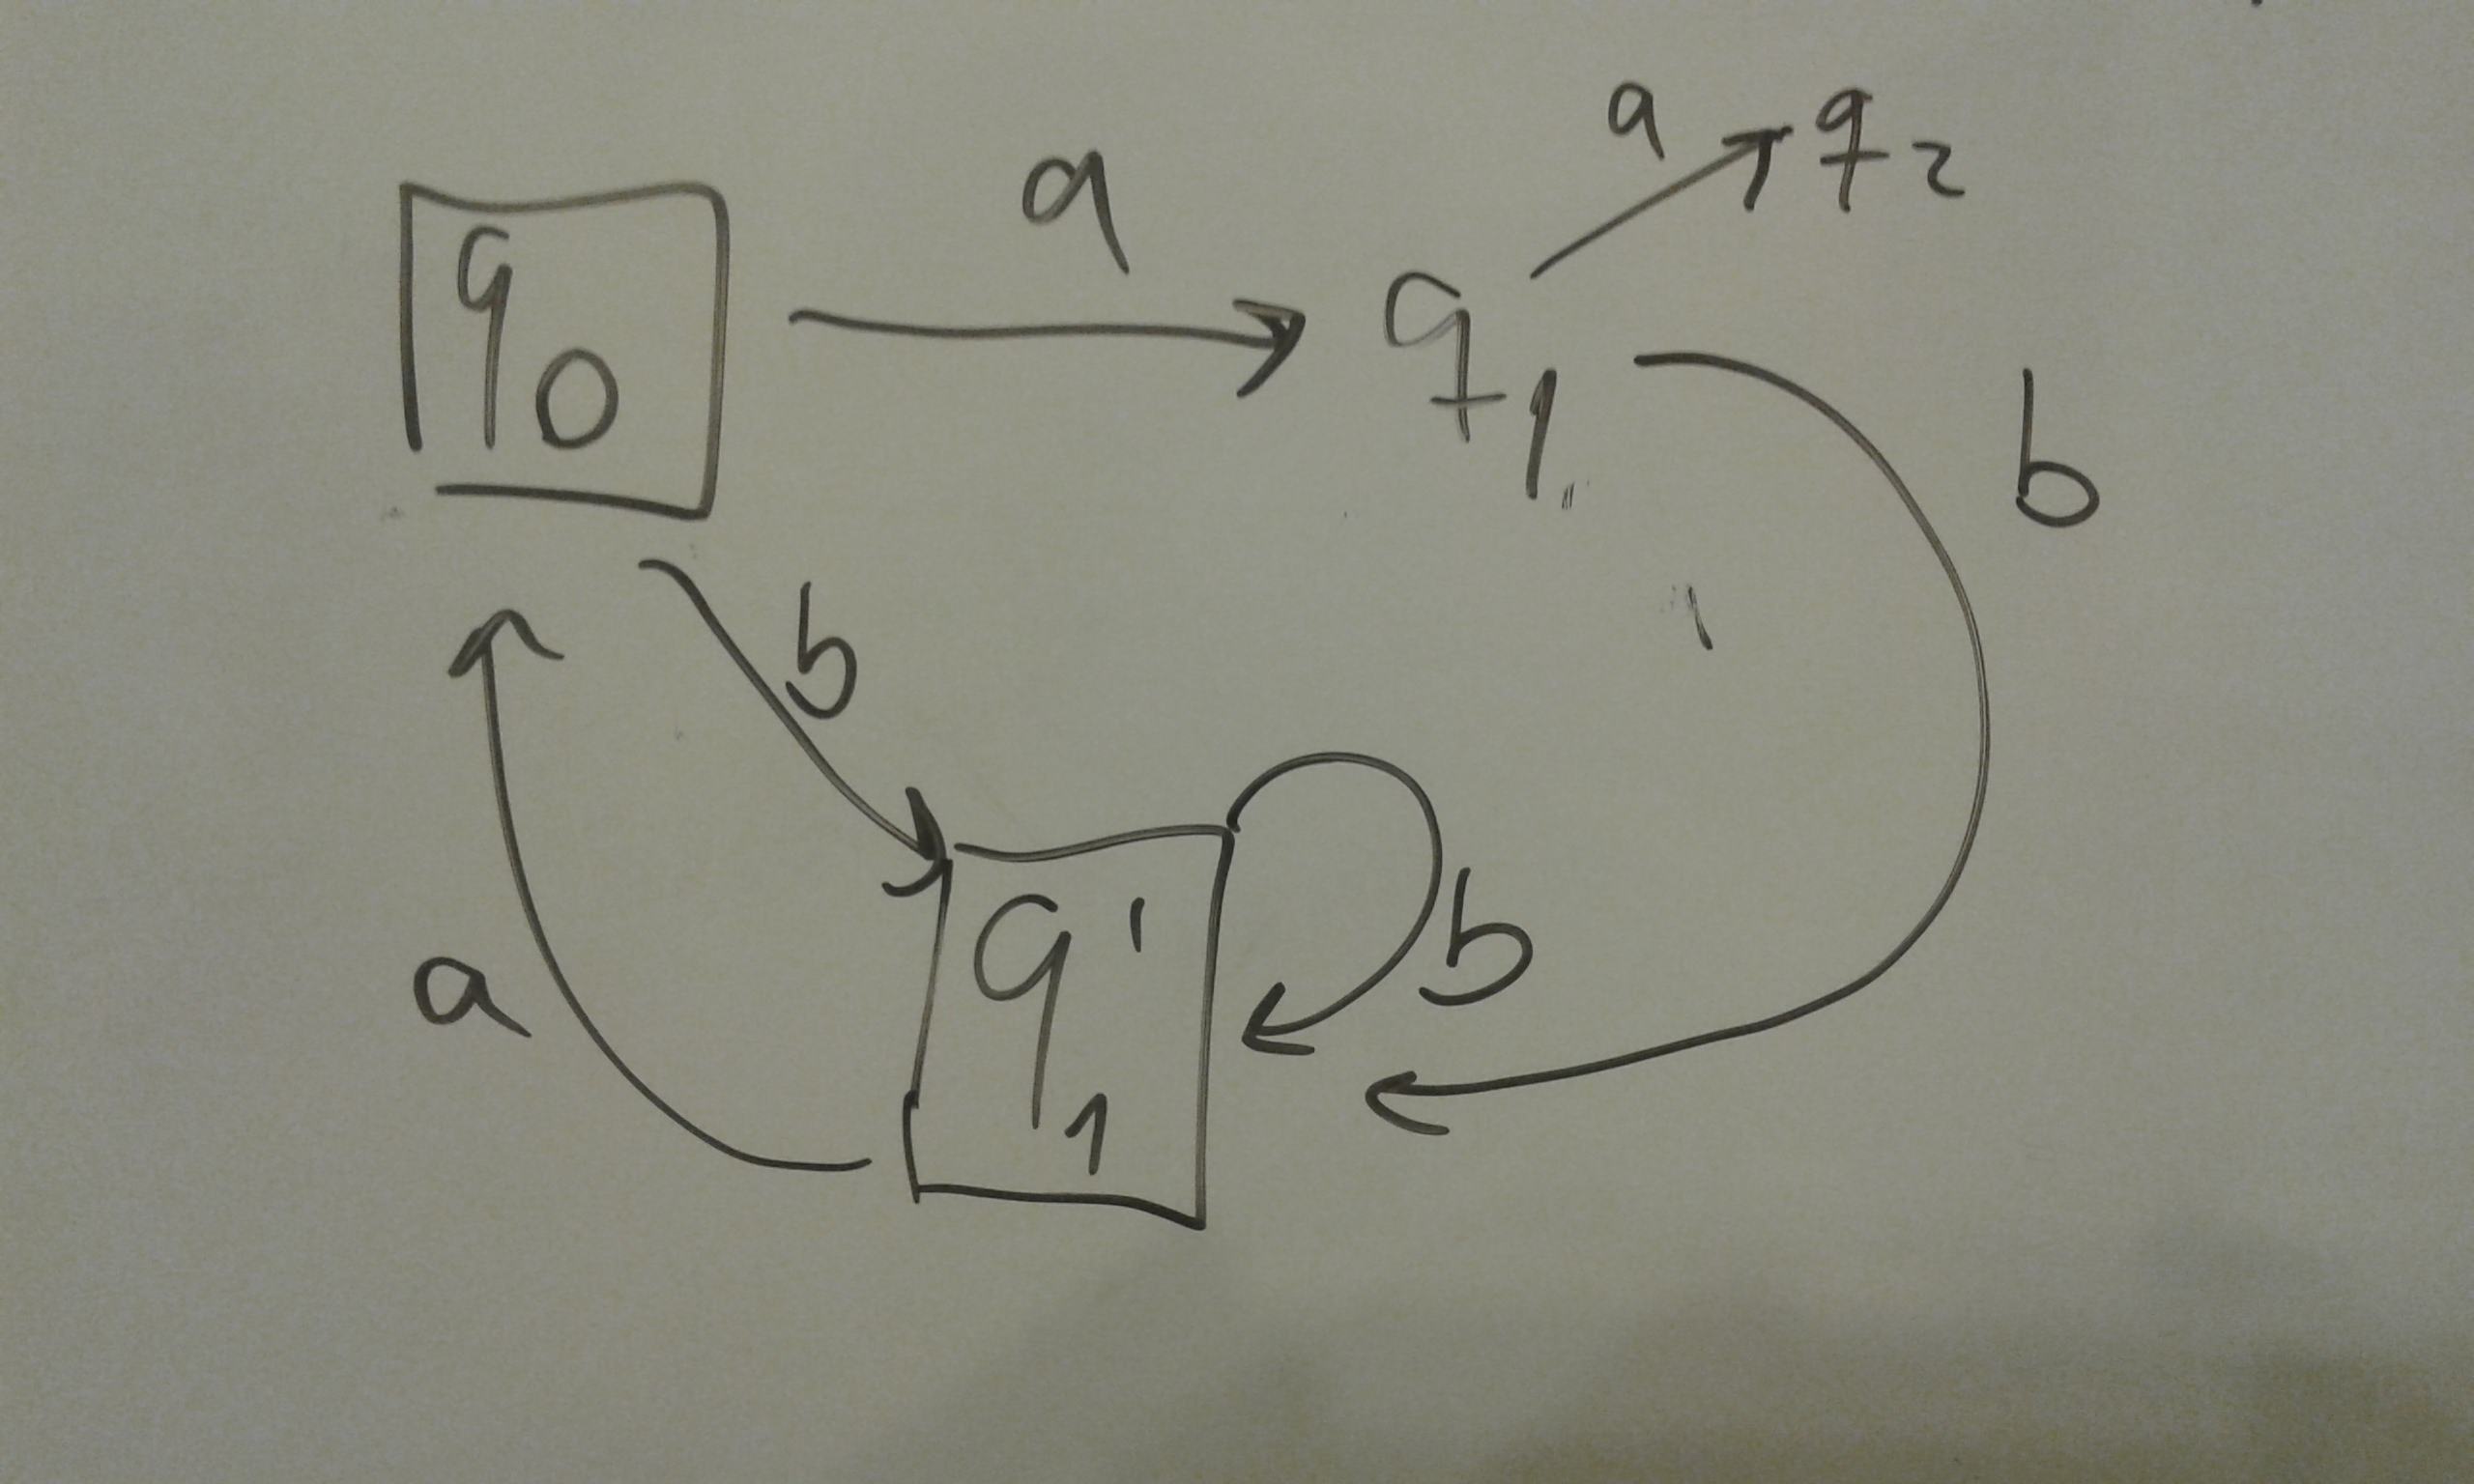
\includegraphics[scale=0.1]{Automatas/1-1}
\end{figure}\

\newpage

\item

 \begin{figure}[h!]
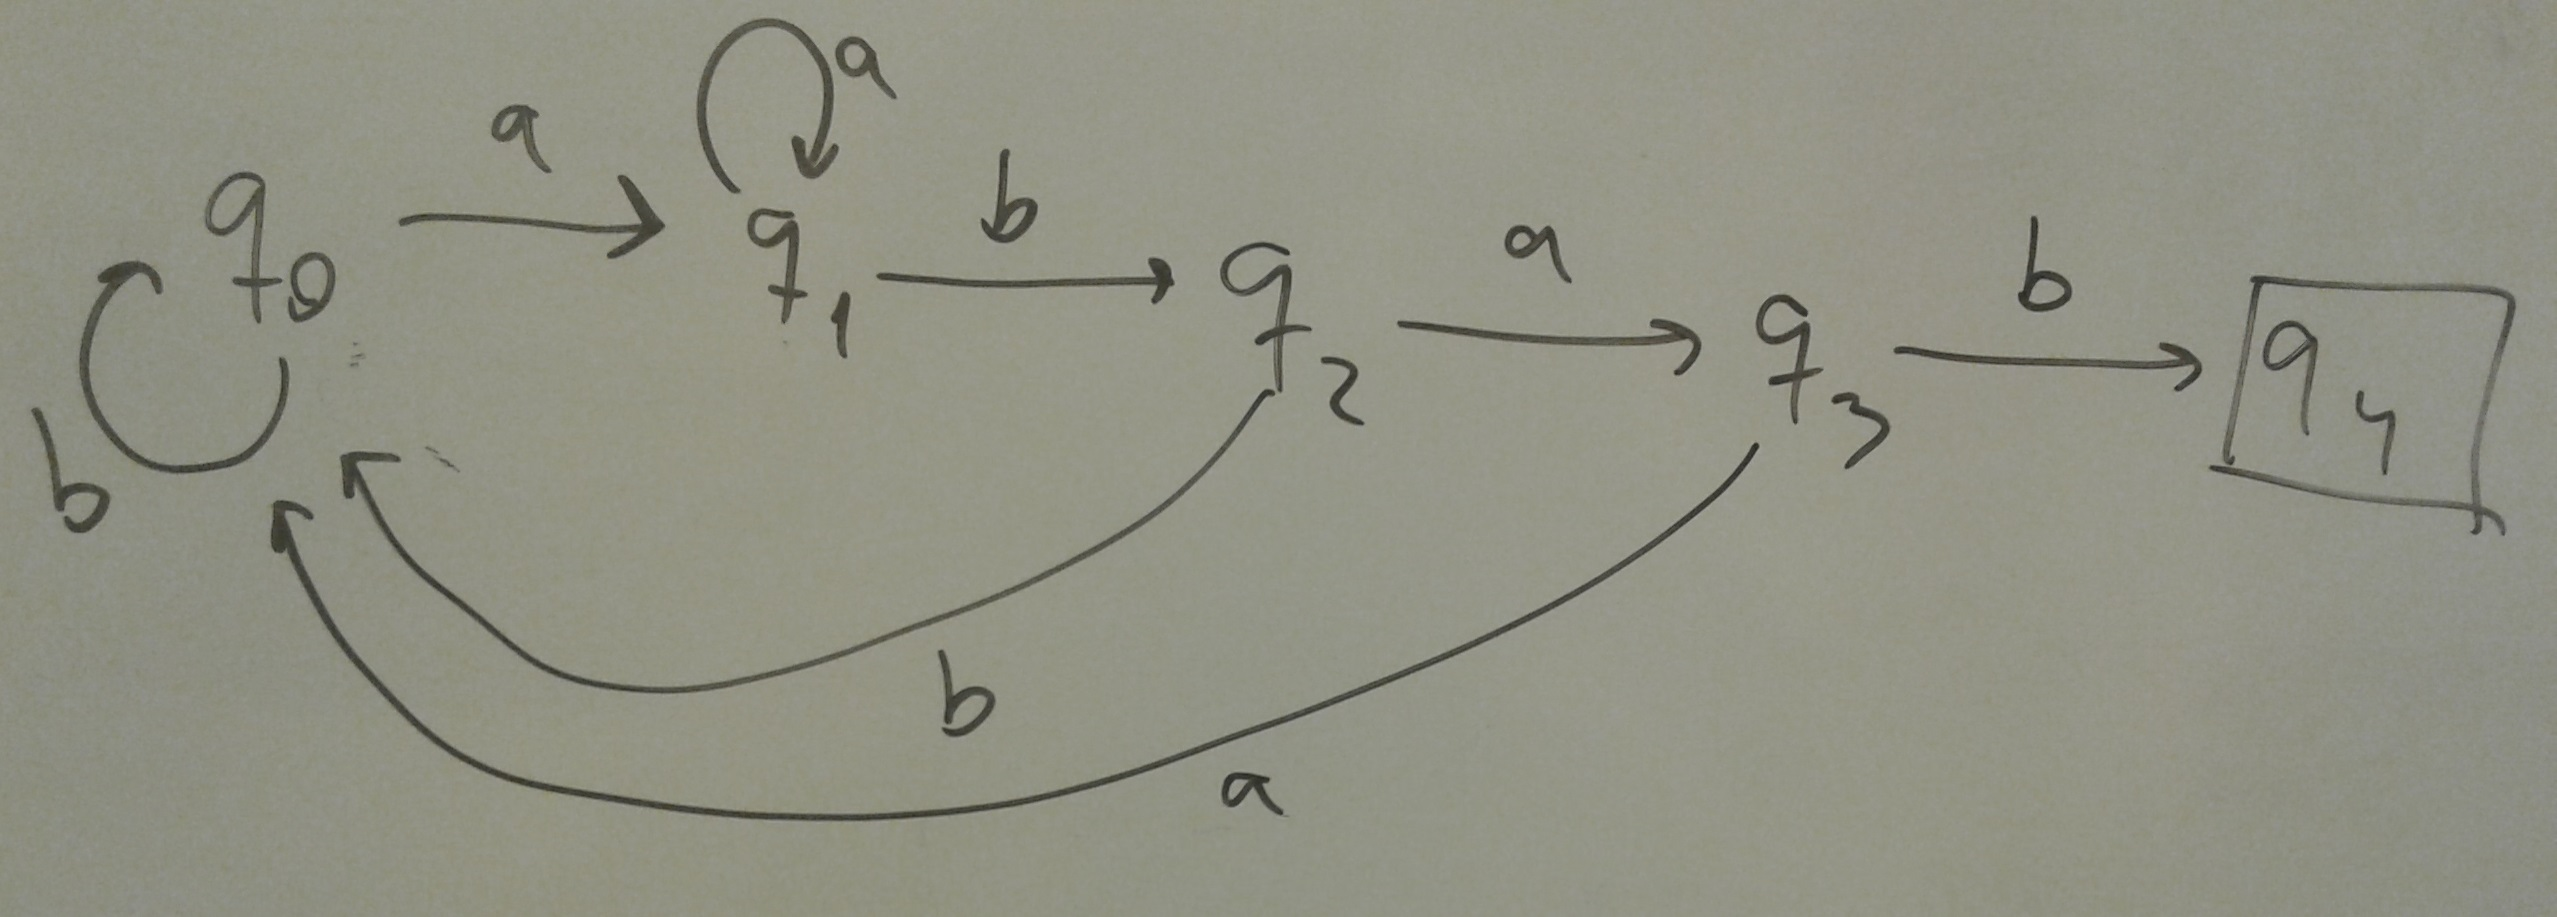
\includegraphics[scale=0.1]{Automatas/1-2}
\end{figure}\

\item 

\begin{figure}[h!]
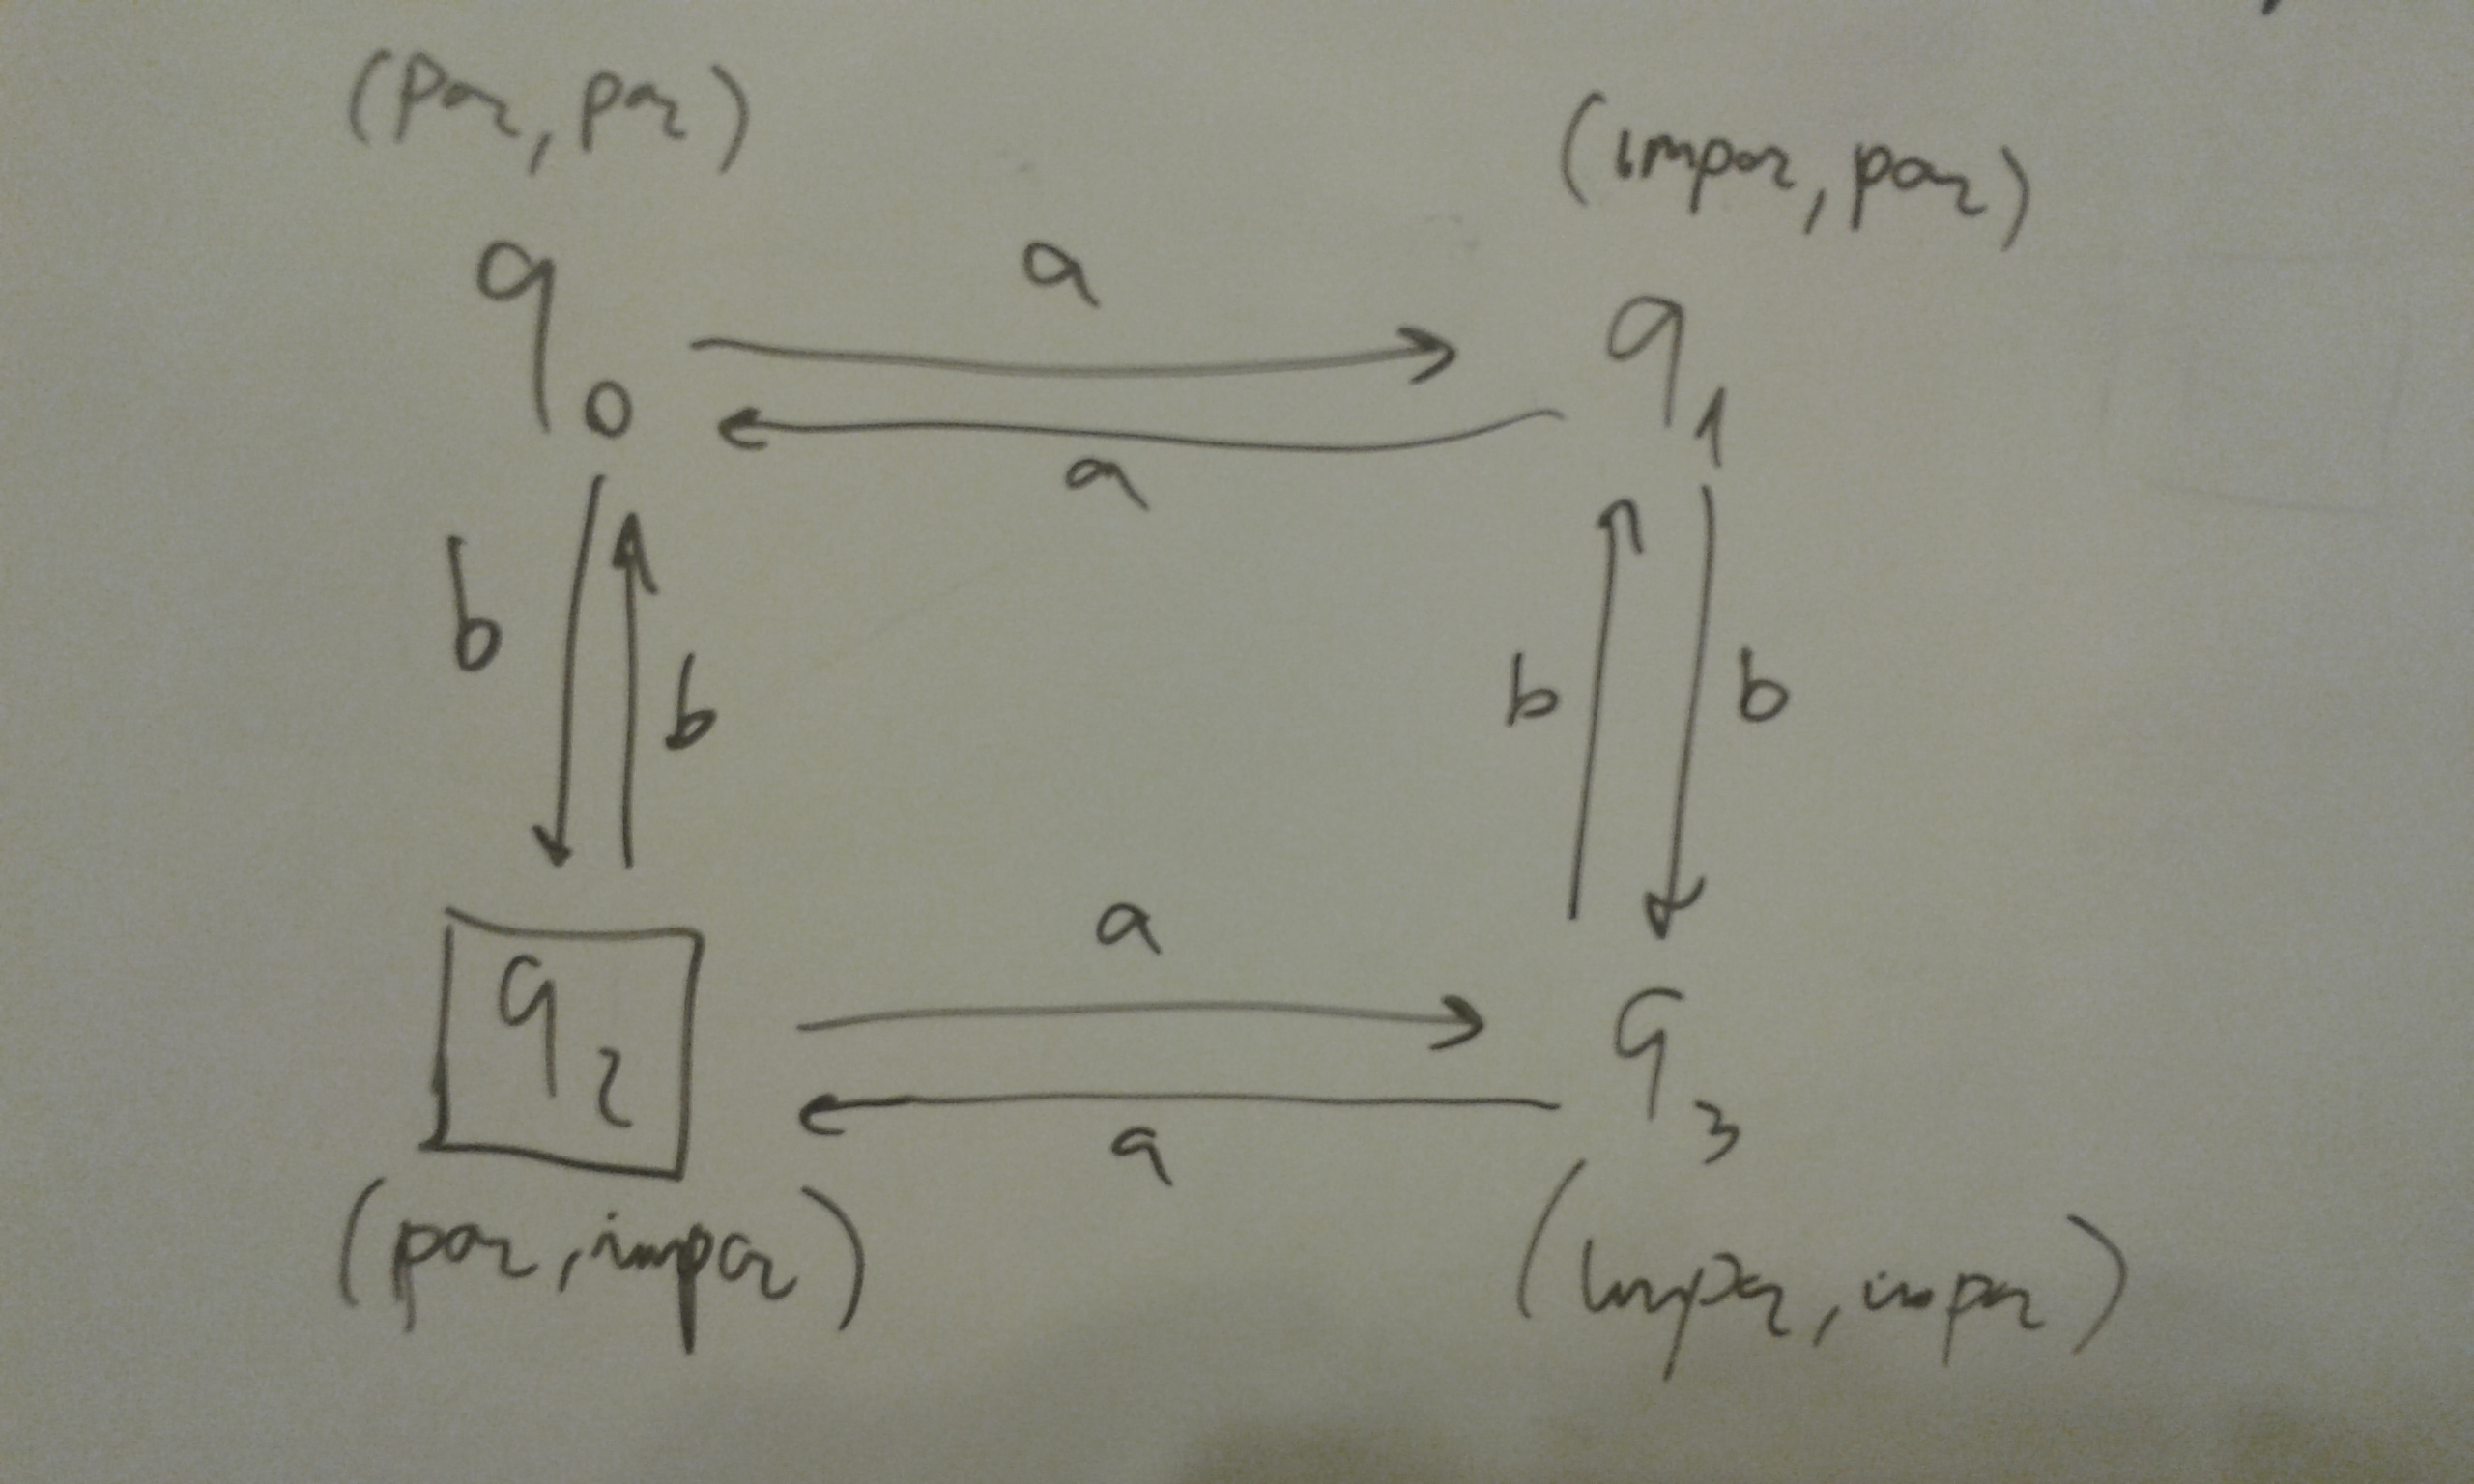
\includegraphics[scale=0.1]{Automatas/1-3}
\end{figure}\

\item 

\begin{figure}[h!]
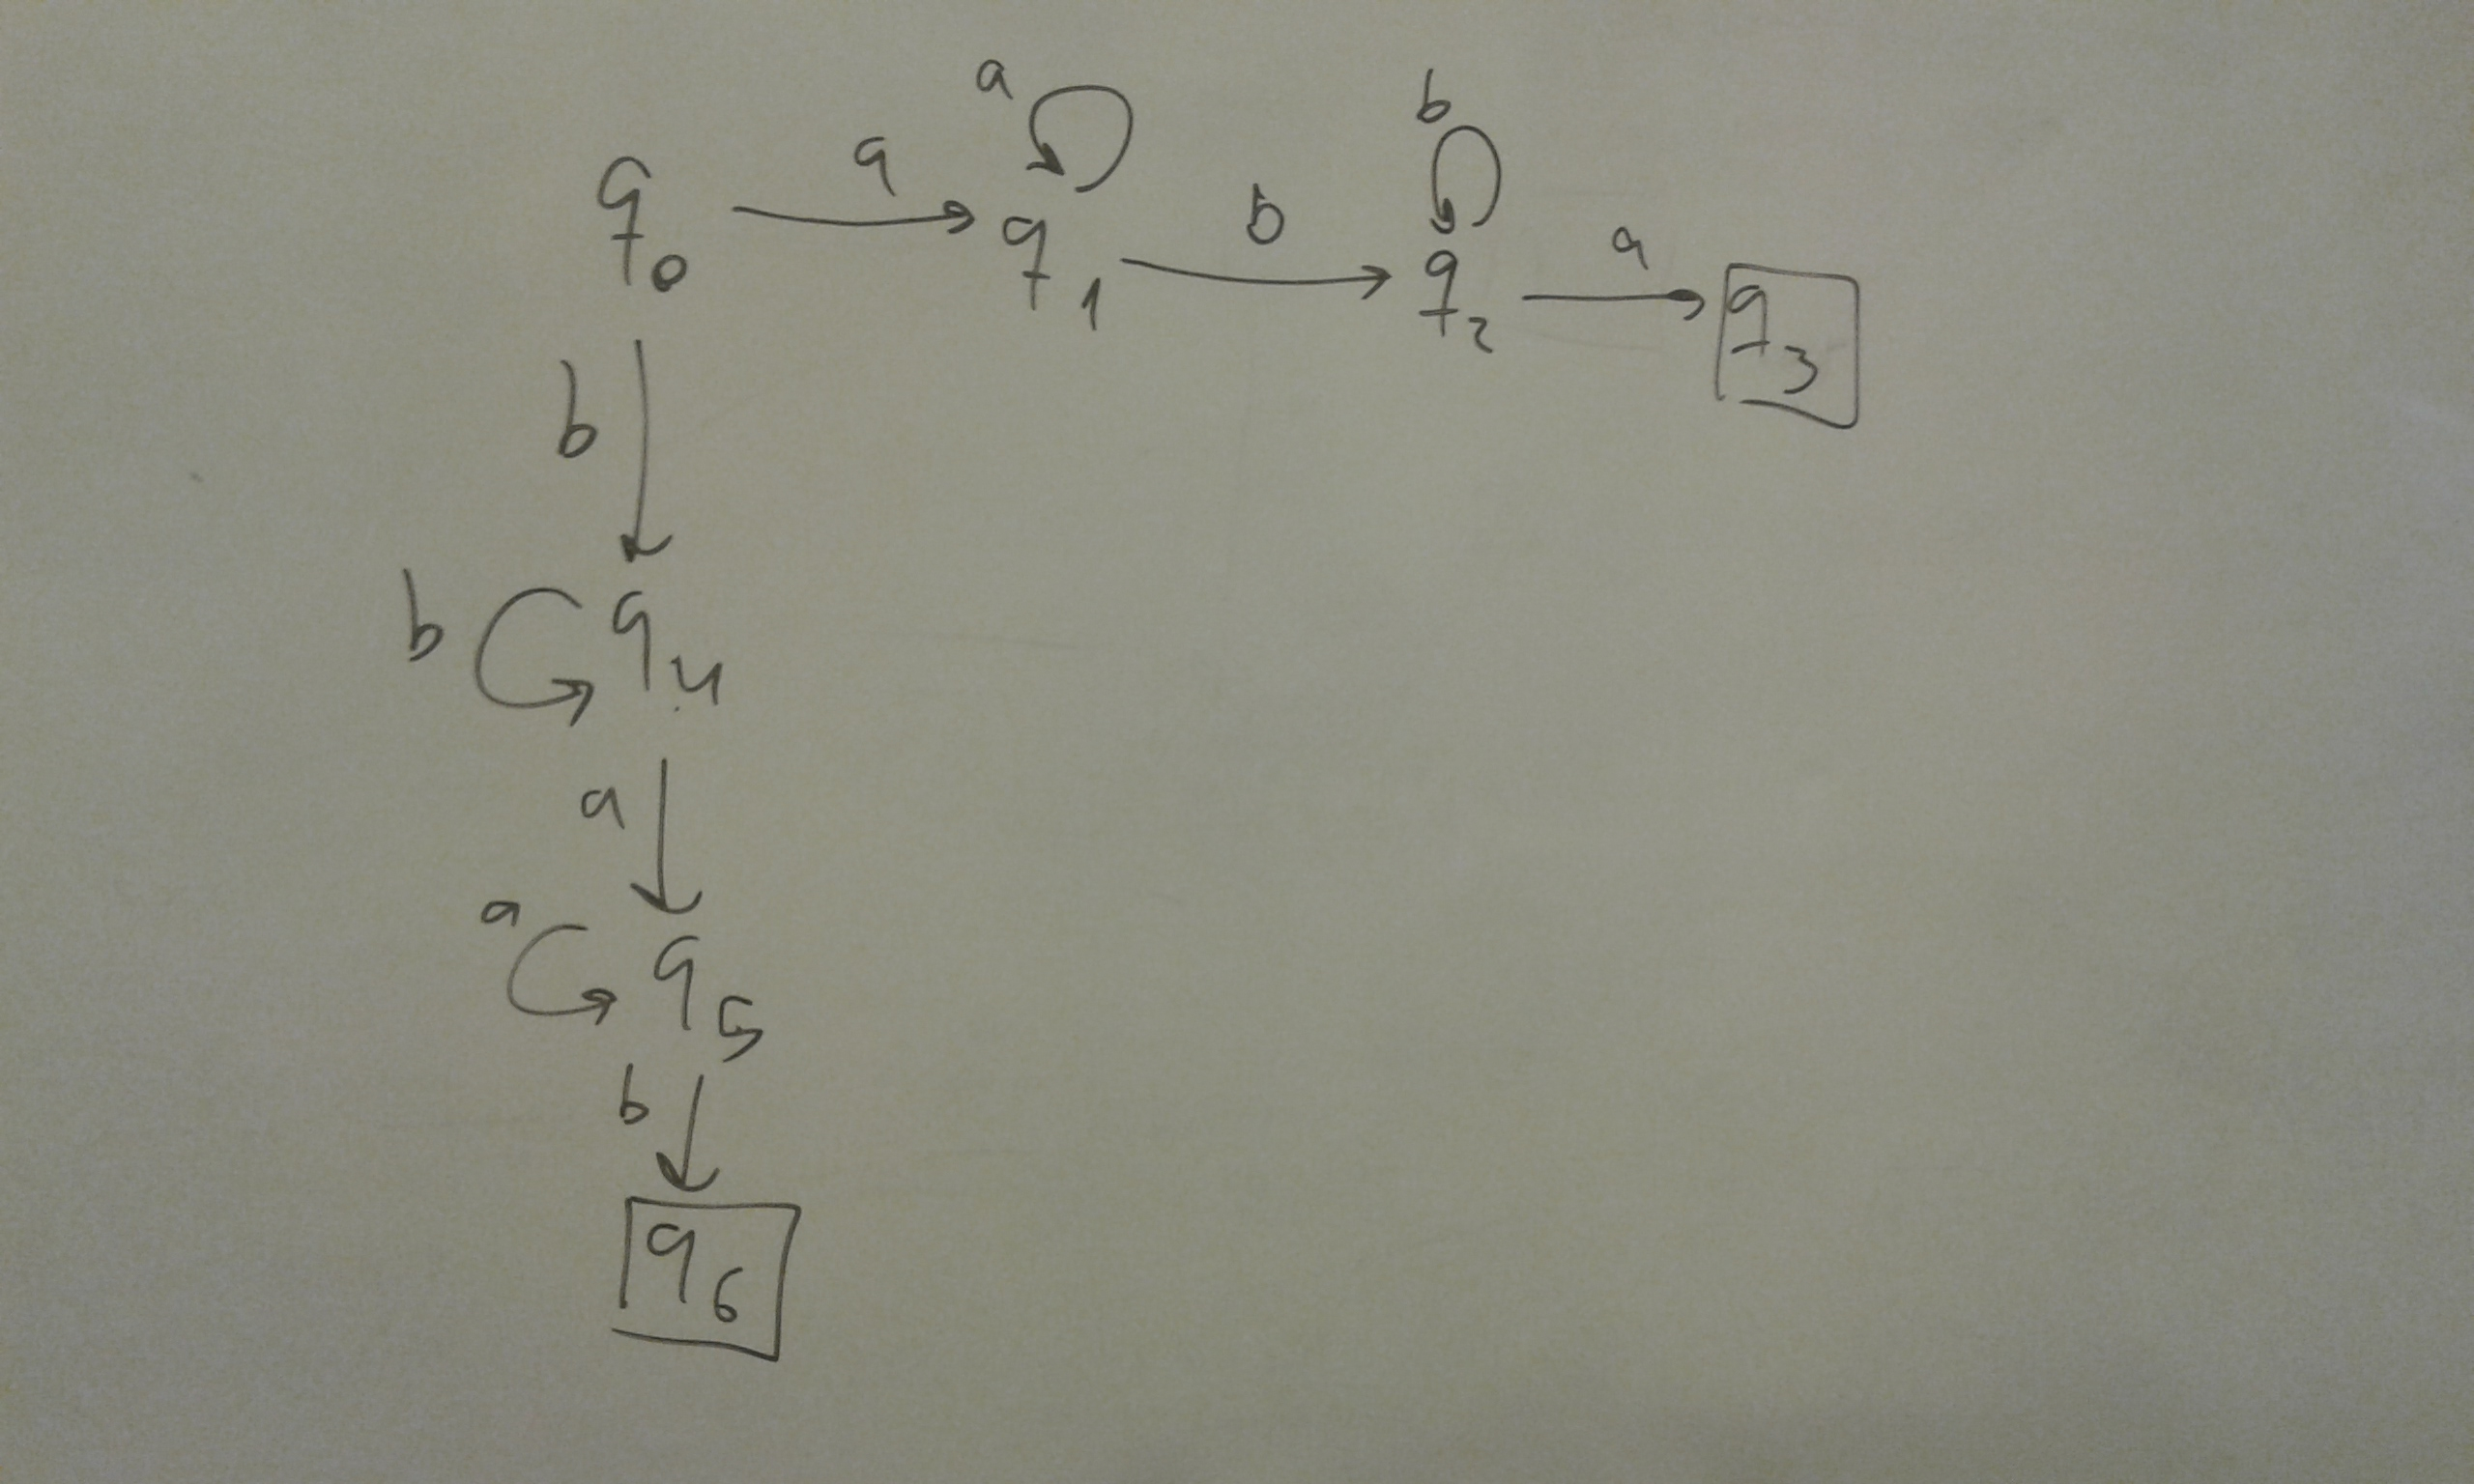
\includegraphics[scale=0.1]{Automatas/1-4}
\end{figure}\
\end{enumerate}
\end{solucion}

\newpage

\begin{ejercicio}{2}
Describe el lenguaje aceptado por cada uno de los siguientes autómatas
\end{ejercicio}
\begin{solucion}\
\begin{enumerate}
\item $M_1$  acepta lo mismo que si quitamos la parte de abajo. Acepta el lenguaje $L(a(ba)^*)$.
\item Como tiene dos estados finales, el lenguaje aceptado es la únión de los lenguajes aceptados por los autómatas que solo tienen uno de los estados finales. Empecemos por $M_{2,1}$ que solo tiene $q_2$ como estado final. Nos podemos quedar con las palabras aceptadas por la parte superior del diagrama. $L(M_{2,1})=L(ab^*a)$. En $M_{2,2}$, pasa lo mismo, así que $L(M_{2,2})=L(b)=\underline{b}$. Por tanto, $L(M_1)=L(a(ba)^*)+\underline{b}=L(a(ba)^*+b)$.

Vamos a resolverlo también aplicando el método de la diapositiva 26.

\item Podemos eliminar cualquier cosa que vaya a $q_3$. $L(M_3)=L(a(ab)^*b)$. 

\item Podemos eliminar cualquier cosa que vaya a $q_3$. $L(M_4)=L((ba)^*+(ab)^*)$
\end{enumerate}
\end{solucion}

\newpage

\begin{ejercicio}{3}
¿Cuáles de las siguientes palabras son aceptadas por el siguiente $\varepsilon$-AFND?
\end{ejercicio}
\begin{solucion}\
\begin{enumerate}
\item No.
\item Sí, $q_0,q_1,q_4,q_5,q_0$.
\item No, si llegas a $q_0$ con $b$, $\hat{\delta}(q_0,b)=\varepsilon-cl(\emptyset)=\emptyset$, así que no cuenta porque no tiene salida. De hecho no puedes leer la letra y te quedas bloqueado.
\item Sí, $q_0,q_1,q_4,q_0,q_1,q_4$.
\end{enumerate}
\end{solucion}

\newpage

\begin{ejercicio}{6}
Para cada una de las siguientes expresiones regulares construir un $\varepsilon$-AFND que
acepte el lenguaje generado por ella:
\begin{enumerate}
\item $(ab)^*(ba)^*+aa^*$.
\item $((ab+aab)^*a^*)^*$.
\item $((a^*b+a^*)^*b)^*$.
\item $(ba + b)^* + (bb + a)^*$.
\end{enumerate}
\end{ejercicio}
\begin{solucion}\
\begin{enumerate}
\item El estado inicial debe ser final para aceptar la palabra vacía.

\begin{figure}[h!]
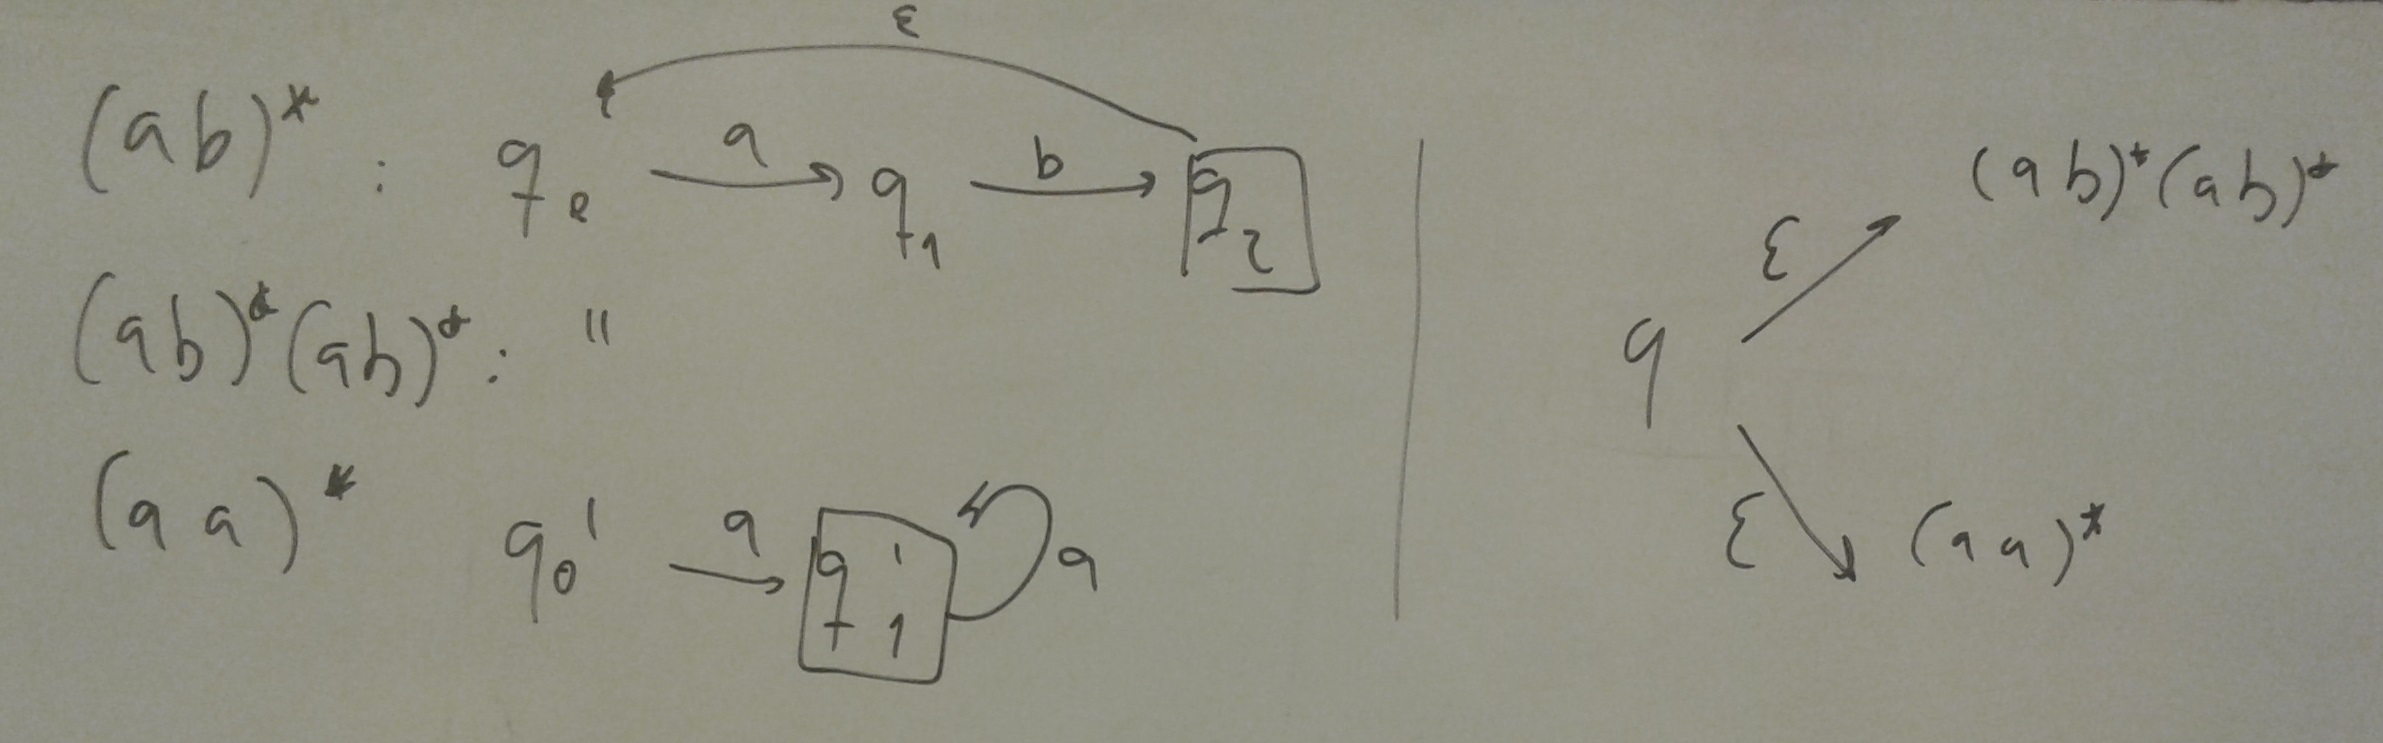
\includegraphics[scale=0.1]{Automatas/6-1}
\end{figure}\

\item 

\begin{figure}[h!]
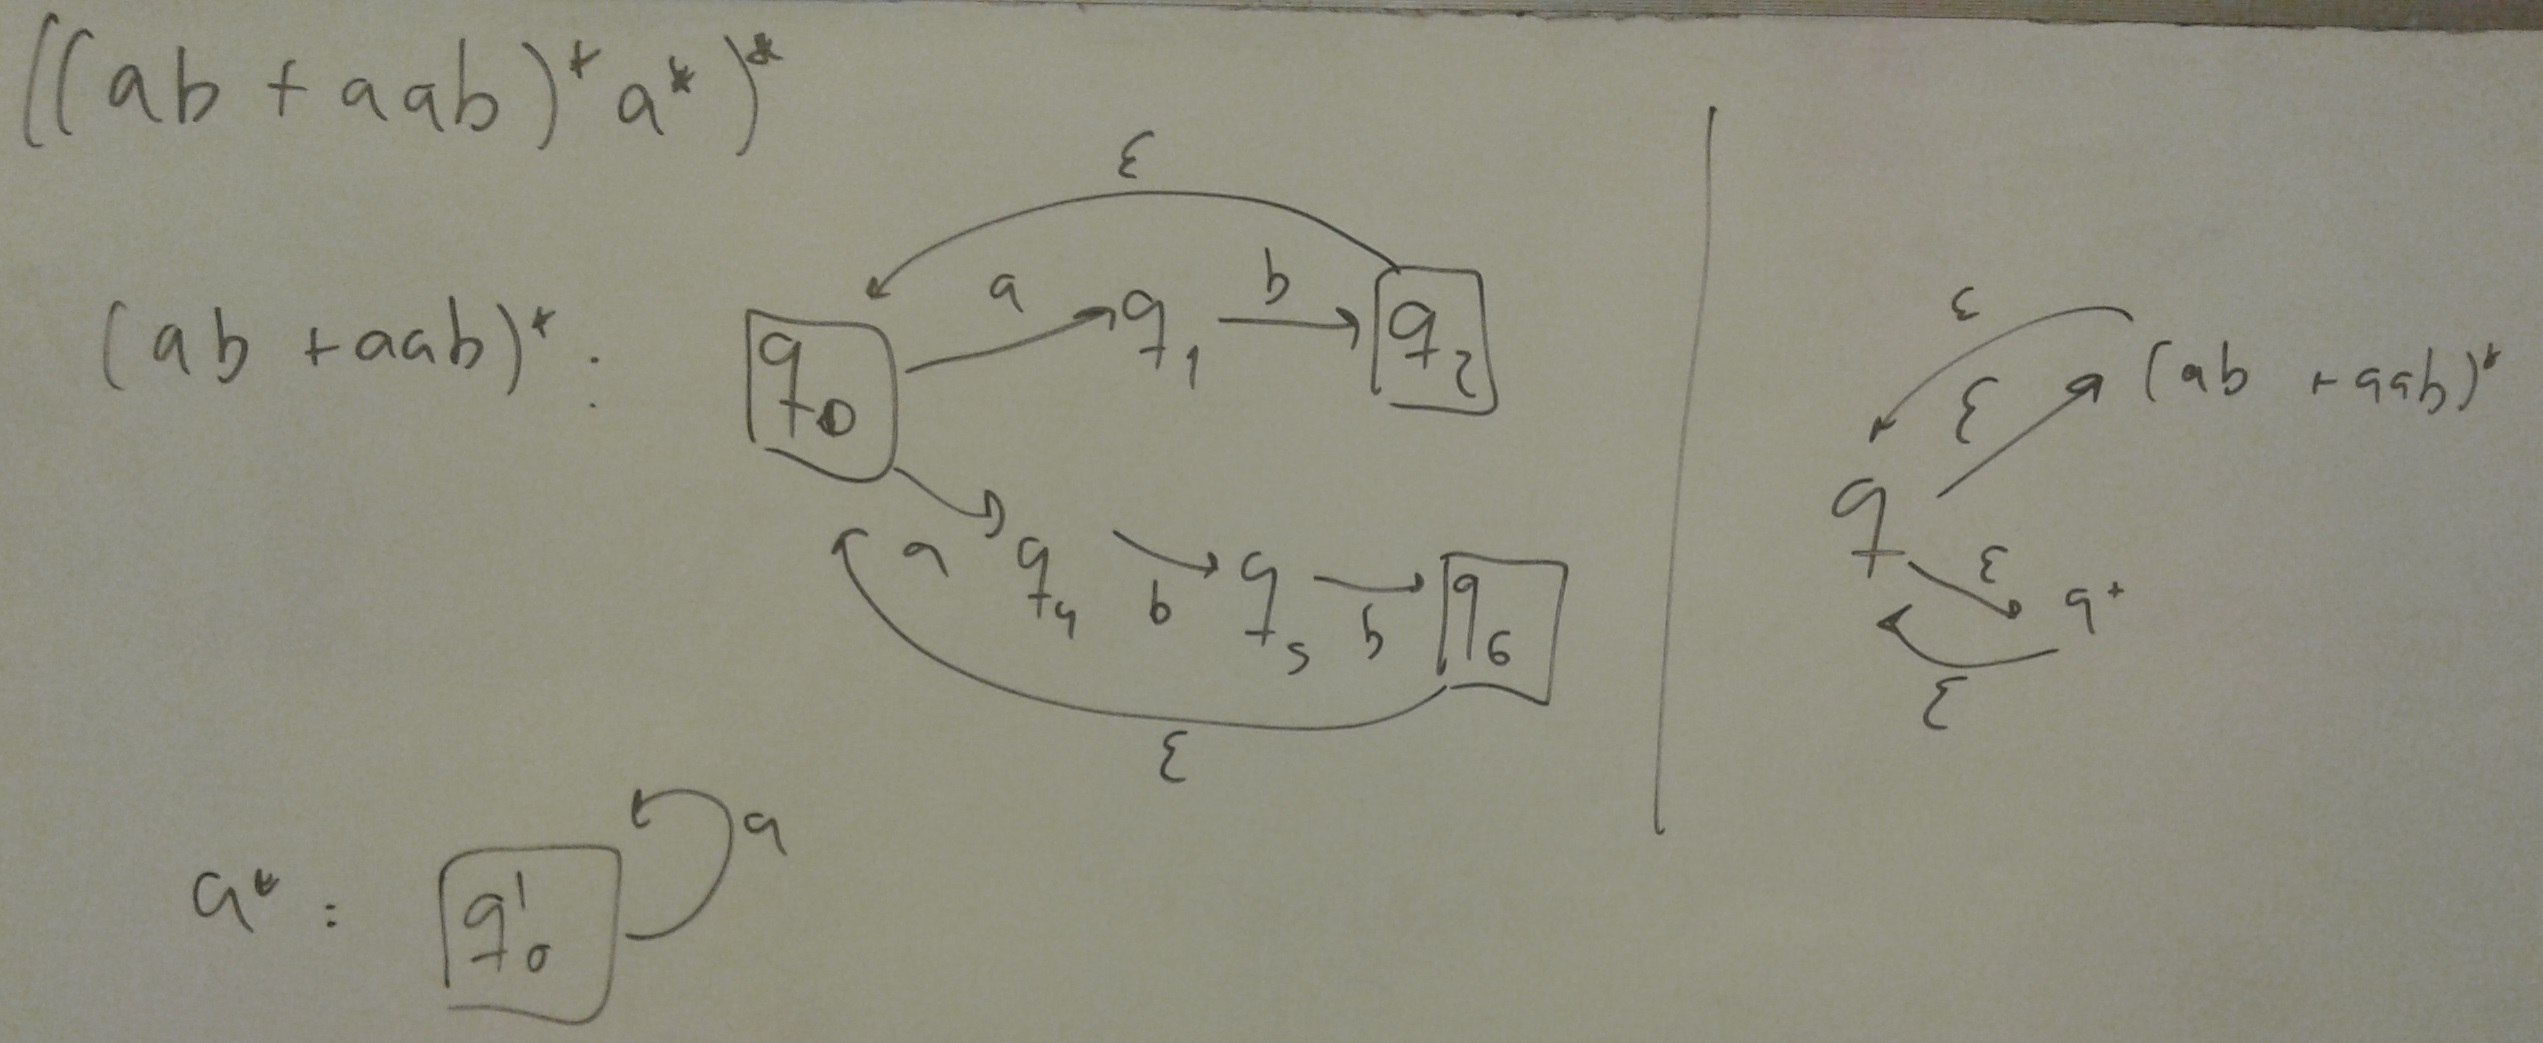
\includegraphics[scale=0.1]{Automatas/6-2}
\end{figure}\
\item

\begin{figure}[h!]
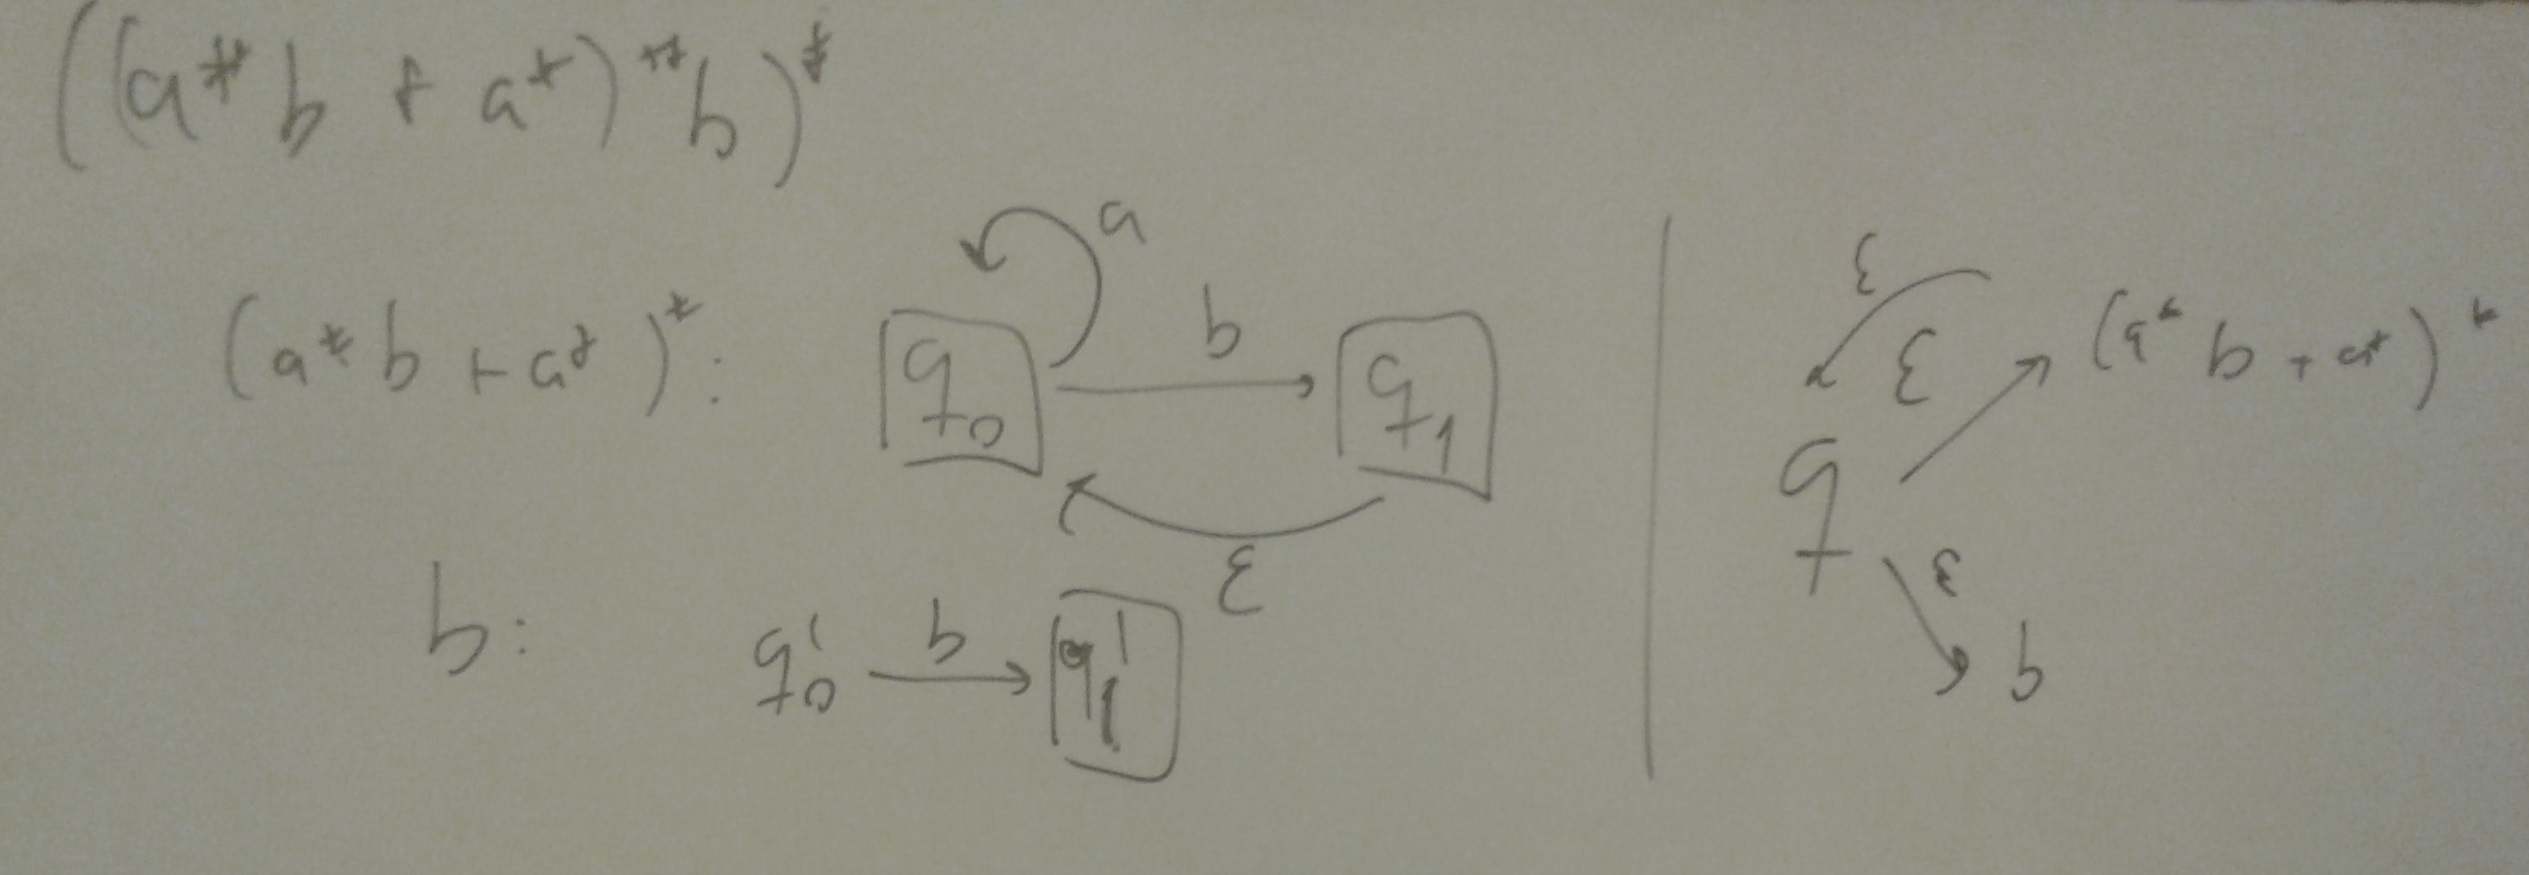
\includegraphics[scale=0.1]{Automatas/6-3}
\end{figure}\

\newpage

\item

\begin{figure}[h!]
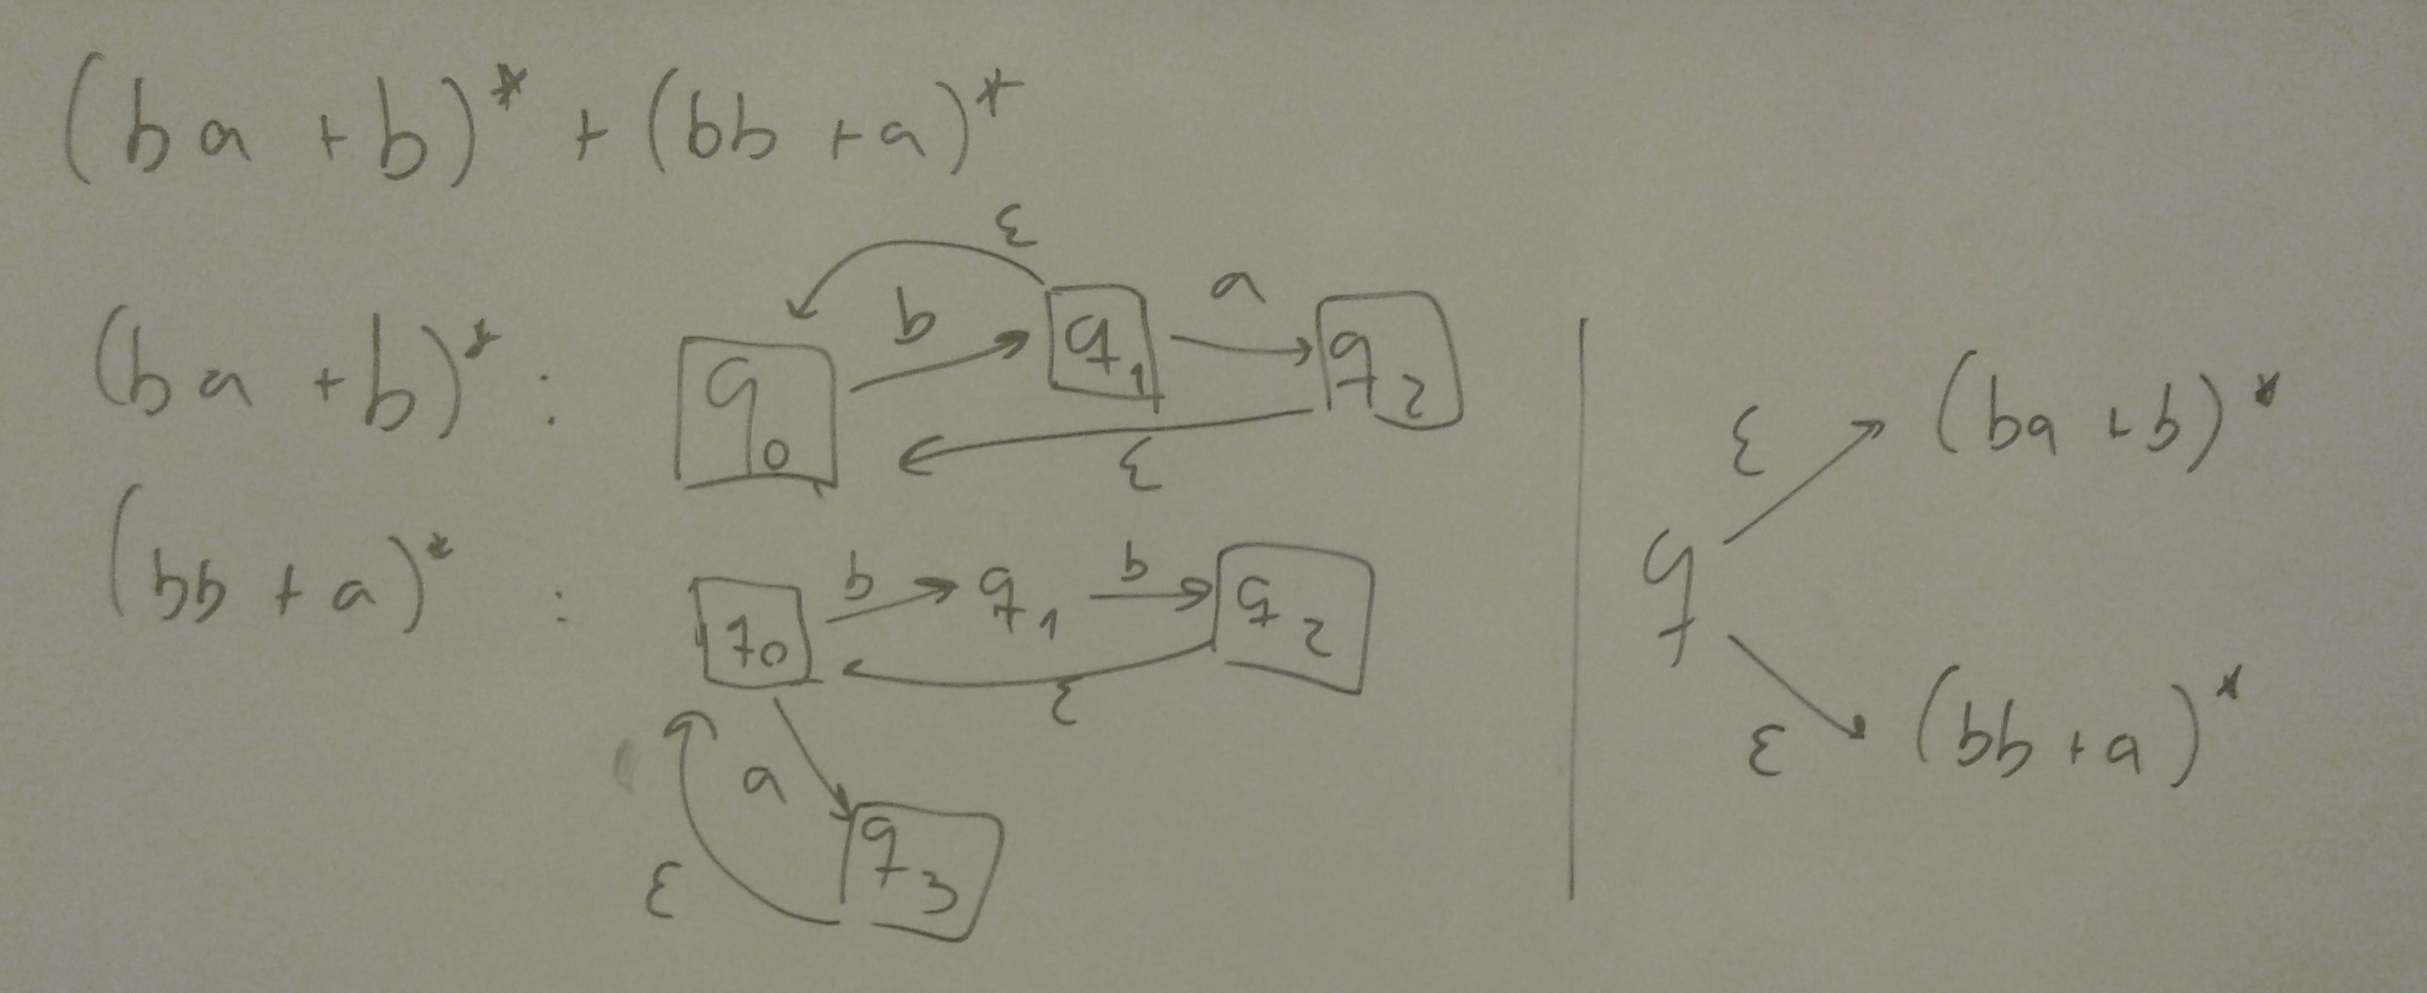
\includegraphics[scale=0.1]{Automatas/6-4}
\end{figure}\ 
\end{enumerate}
\end{solucion}

\newpage

\begin{ejercicio}{7}
Sea $L = L(((aa) + (aaa))^*)$. Encontrar un AFD que acepte $L$.
\end{ejercicio}
\begin{solucion}\

\begin{figure}[h!]
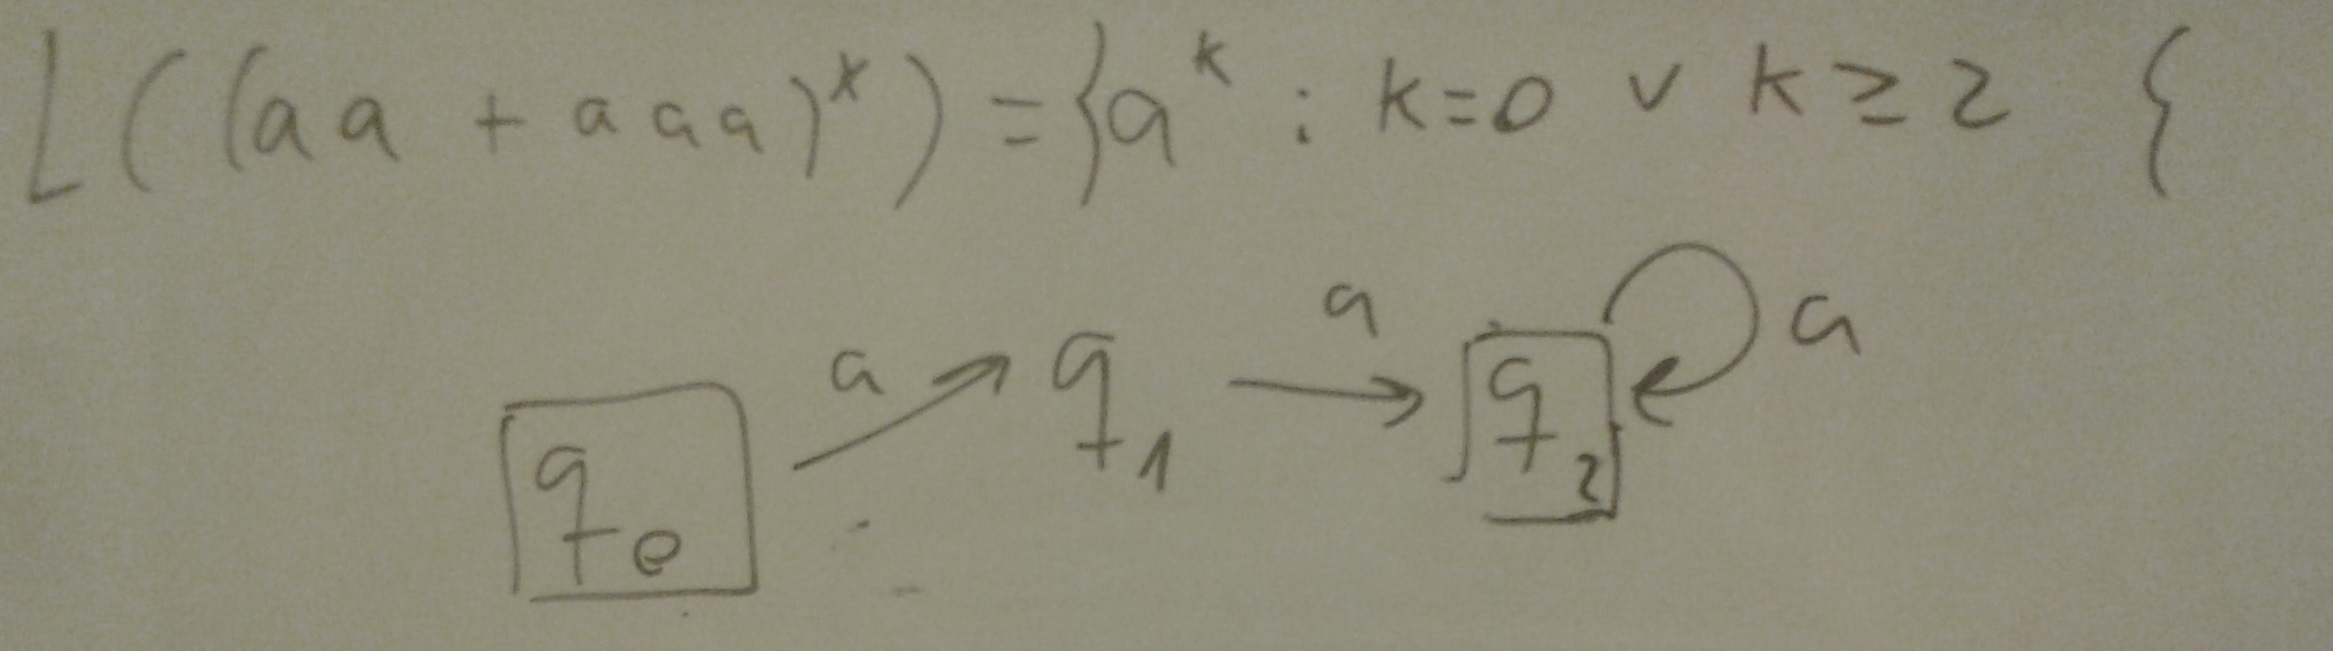
\includegraphics[scale=0.2]{Automatas/7}
\end{figure}\
\end{solucion}

\newpage

\begin{ejercicio}{8}
Condieremos el alfabeto
$$\Sigma_3 = \left\{\begin{bmatrix}
0\\
0\\
0
\end{bmatrix},\begin{bmatrix}
1\\
0\\
0
\end{bmatrix},\begin{bmatrix}
0\\
1\\
0
\end{bmatrix},\dots,\begin{bmatrix}
1\\
1\\
1
\end{bmatrix}\right\}$$

formado por todas la columnas de 0's y 1's de altura 3. Una palabra sobre $\Sigma_3$ puede identificarse
con una matriz de 3 filas formada por 0's y 1's, cada una de las cuales puede considerarse un
número natural en notación binaria. Probar que el lenguaje
$$B = \{w \in \Sigma^*_3: \text{la fila inferior es la suma de las dos filas superiores}\}$$
es regular.
\end{ejercicio}
\begin{solucion}
Hay que pensarlo con cuidao. Cada columna se corresponde a las columnas de una suma de números binarios. El autómata comprueba si la suma está bien hecha. Ojo con las llevadas. El autómata lee de izquiera a derecha así que hay que invertir los números. 
\end{solucion}
\newpage

\begin{ejercicio}{9}
Condieremos el alfabeto
$$\Sigma_2 = \left\{\begin{bmatrix}
0\\
0\\
\end{bmatrix},\begin{bmatrix}
1\\
0\\
\end{bmatrix},\begin{bmatrix}
0\\
1\\
\end{bmatrix},\begin{bmatrix}
1\\
1\\
\end{bmatrix}\right\}$$
formado por todas la columnas de 0's y 1's de altura 2. Una palabra sobre $\Sigma_2$ puede identificarse
con una matriz de 2 filas formada por 0's y 1's, cada una de las cuales puede considerarse un
número natural en notación binaria. Probar que los siguientes lenguajes son regulares:
\begin{enumerate}
\item $C = \{w \in \Sigma^*_2
: \text{la fila inferior es la superior multiplicada por } 3\}$. 
\item $D = \{w \in \Sigma^*_2
: \text{la fila inferior es menor que la superior}\}$.  
\end{enumerate}
\end{ejercicio}
\begin{solucion}


\begin{figure}[h!]
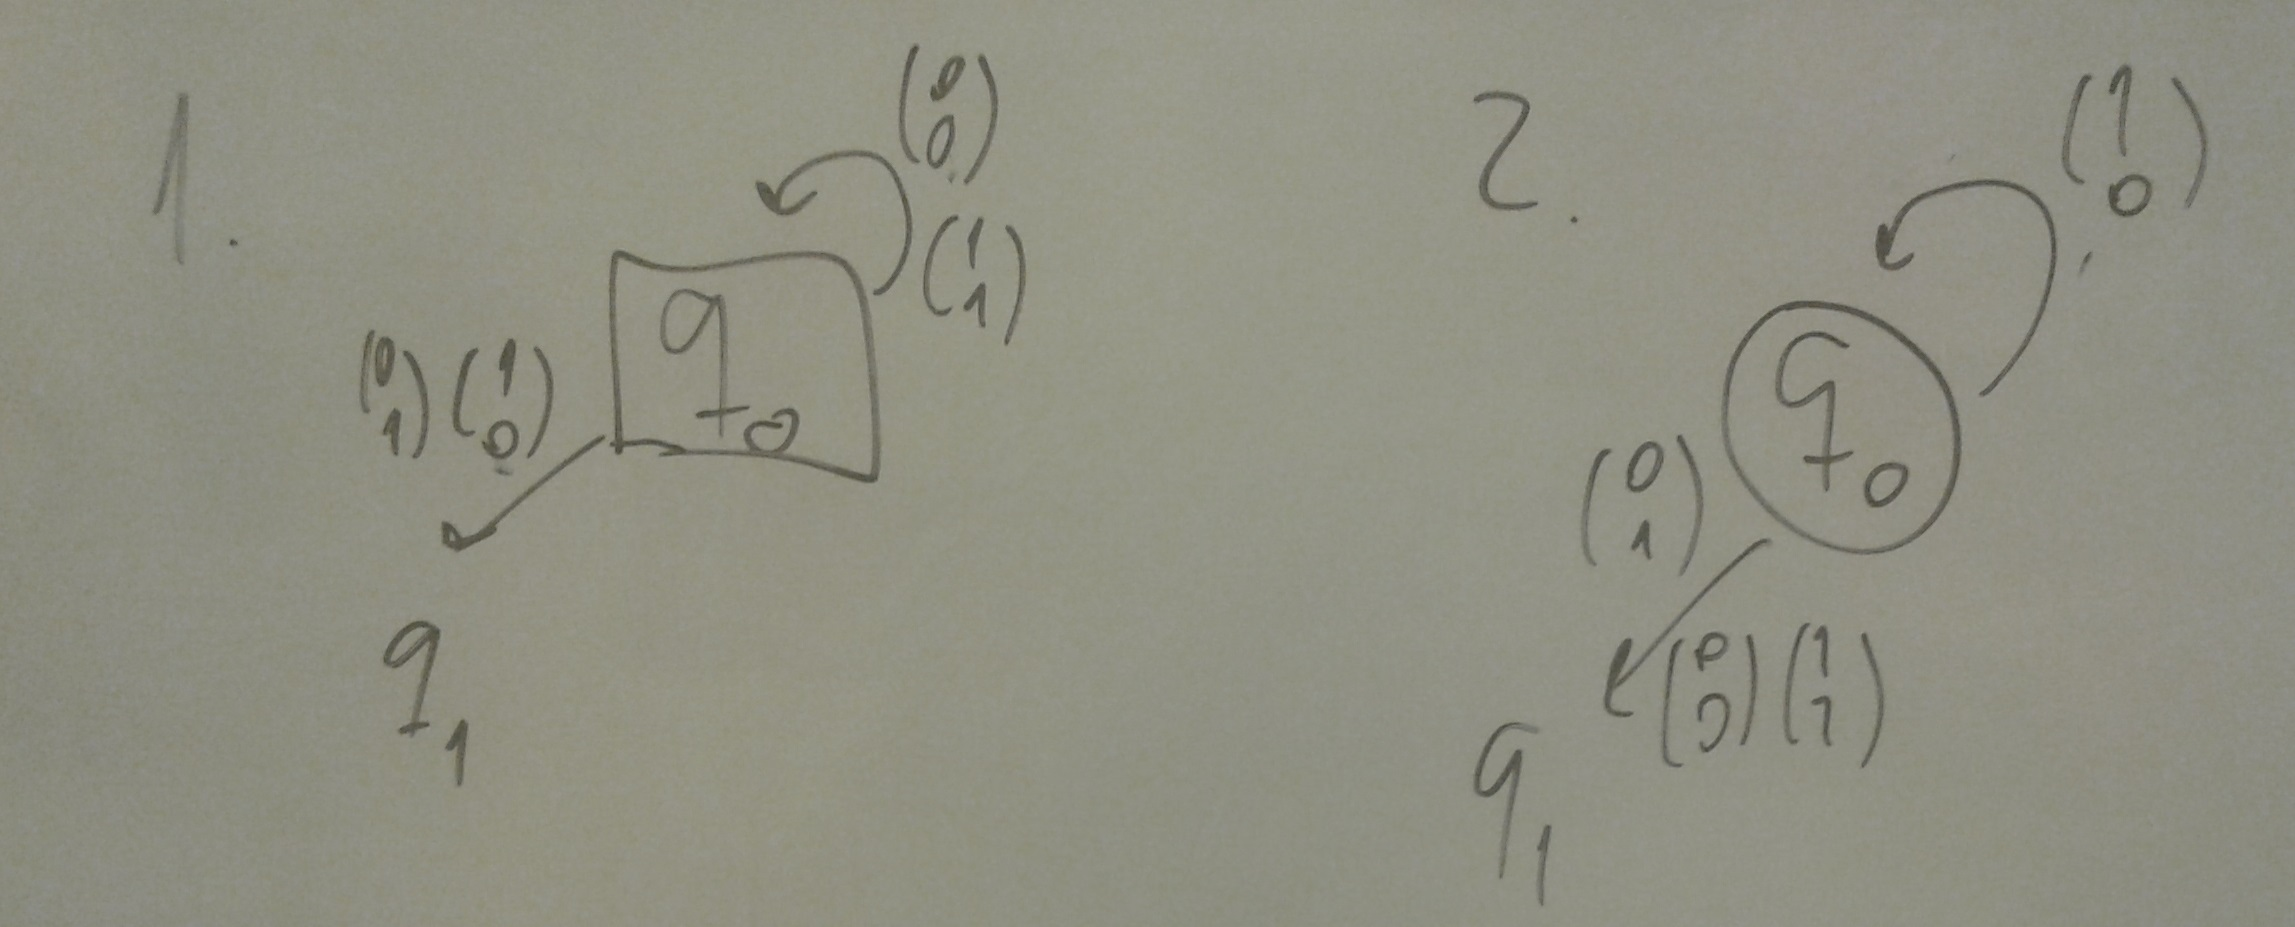
\includegraphics[scale=0.1]{Automatas/9}
\end{figure}\
\end{solucion}
\newpage

\begin{ejercicio}{11}
Construir un AFD equivalente al siguiente AFND:
\end{ejercicio}
\begin{solucion}\

\begin{figure}[h!]
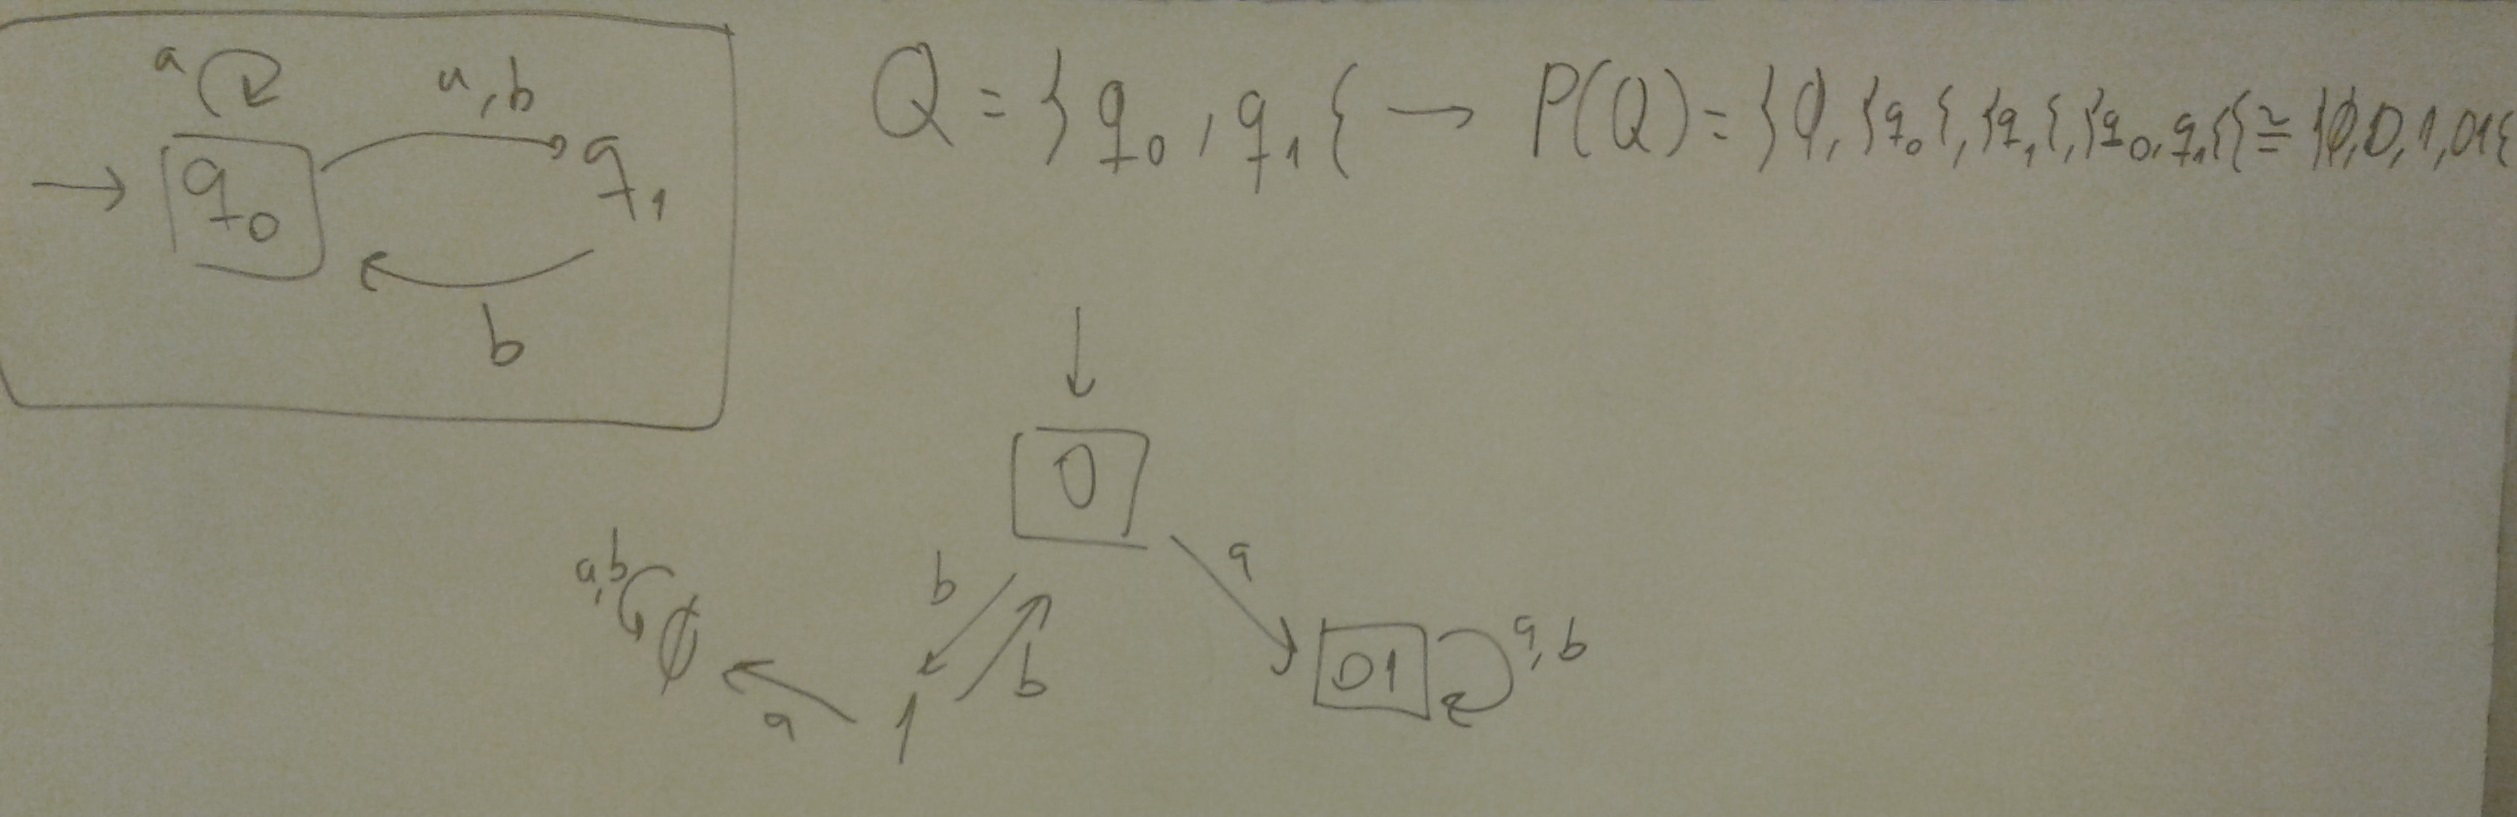
\includegraphics[scale=0.2]{Automatas/11}
\end{figure}\
\end{solucion}

\newpage

\begin{ejercicio}{12}
Construir un AFD equivalente al siguiente $\varepsilon$-AFND:
\end{ejercicio}
\begin{solucion}
Tener en cuenta que hay que hacer el $\varepsilon-$cl, es decir, ver si se puede llegar a algún sitio con un $\varepsilon$-movimiento.

\begin{figure}[h!]
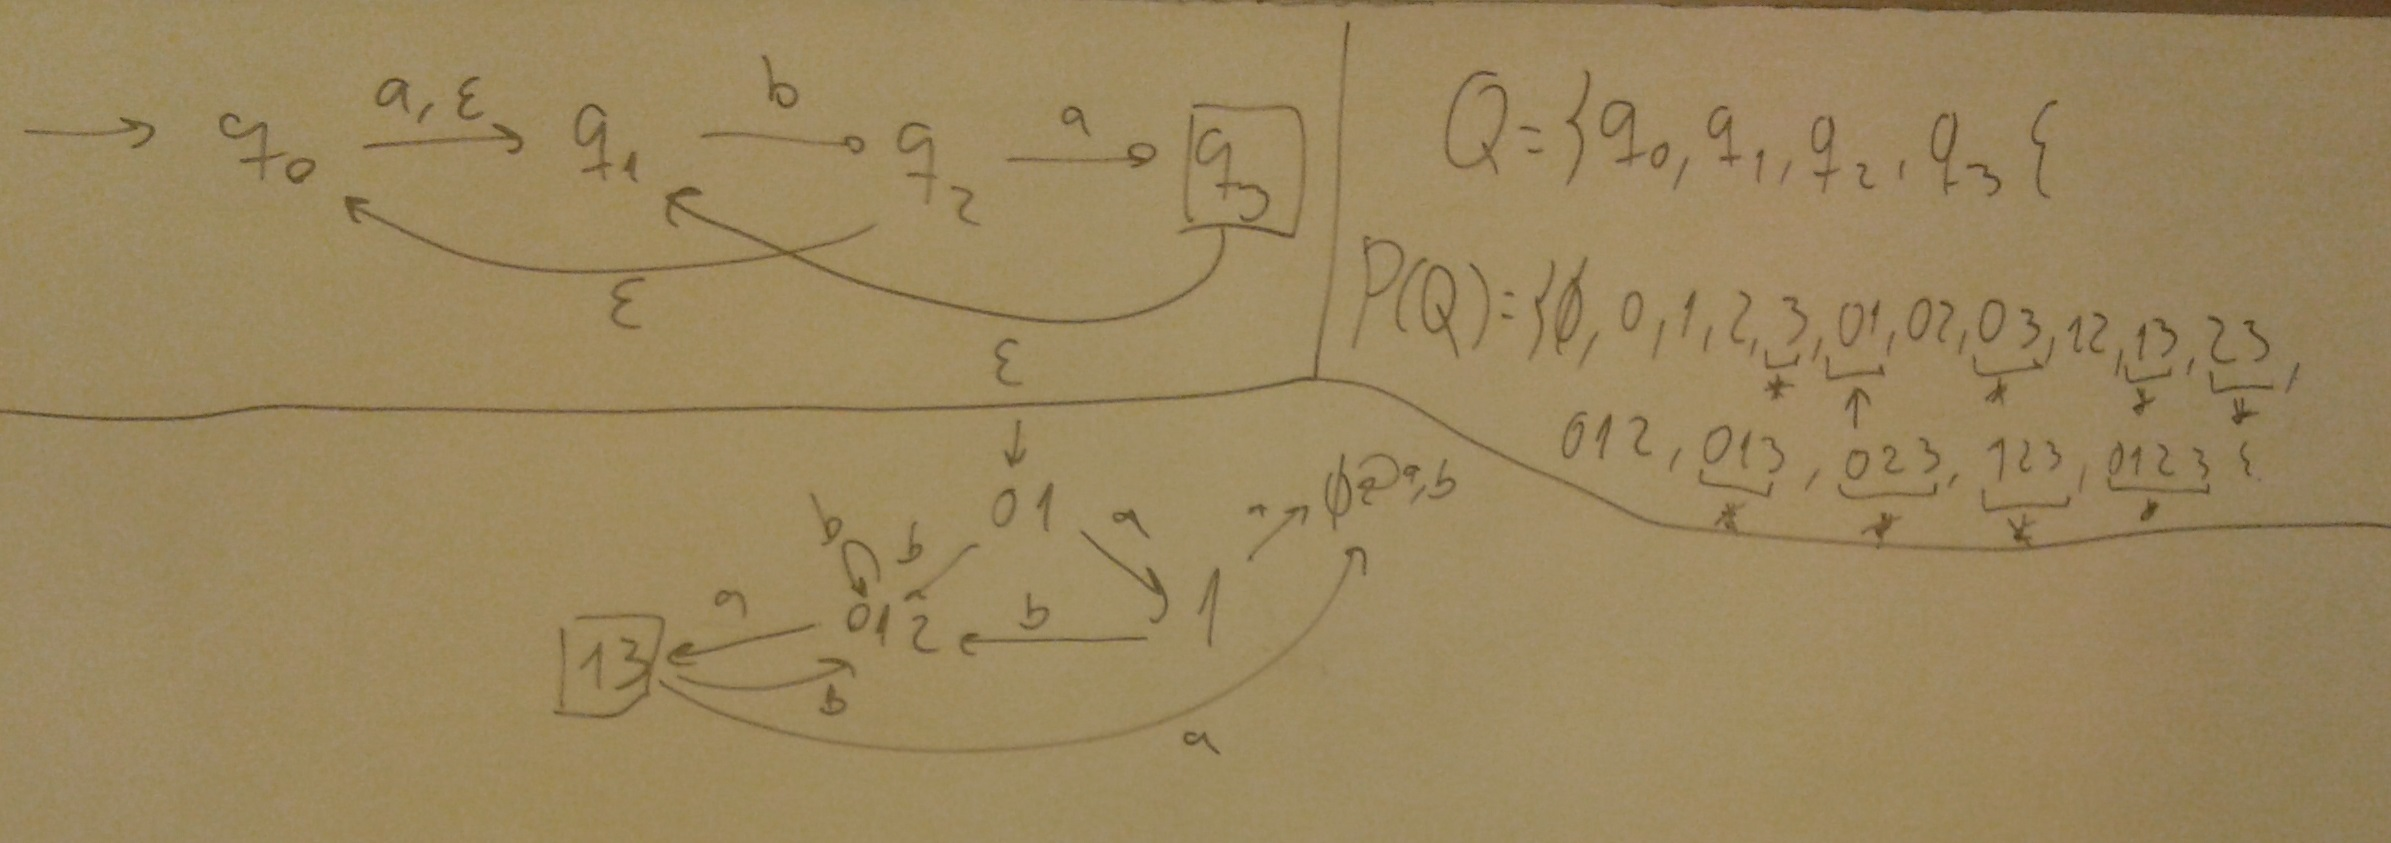
\includegraphics[scale=0.2]{Automatas/12}
\end{figure}\
\end{solucion}

\newpage

\begin{ejercicio}{13}
Consideremos la gramática regular:
\begin{align*}
&S \rightarrow xN\\
&S \rightarrow x\\
&N \rightarrow yM\\
&N \rightarrow y\\
&M \rightarrow zN\\
&M \rightarrow z
\end{align*}
donde $S$ es el símbolo inicial, $\{x, y, z\}$ son terminales y $\{S,N,M\}$ variables. Se pide:
\begin{enumerate}
\item Construir un $\varepsilon$-AFND que acepte el lenguaje generado por $\Gamma$.
\item Encontrar una expresión regular que genere el lenguaje generado por $\Gamma$.
\end{enumerate}
\end{ejercicio}
\begin{solucion}\

\begin{figure}[h!]
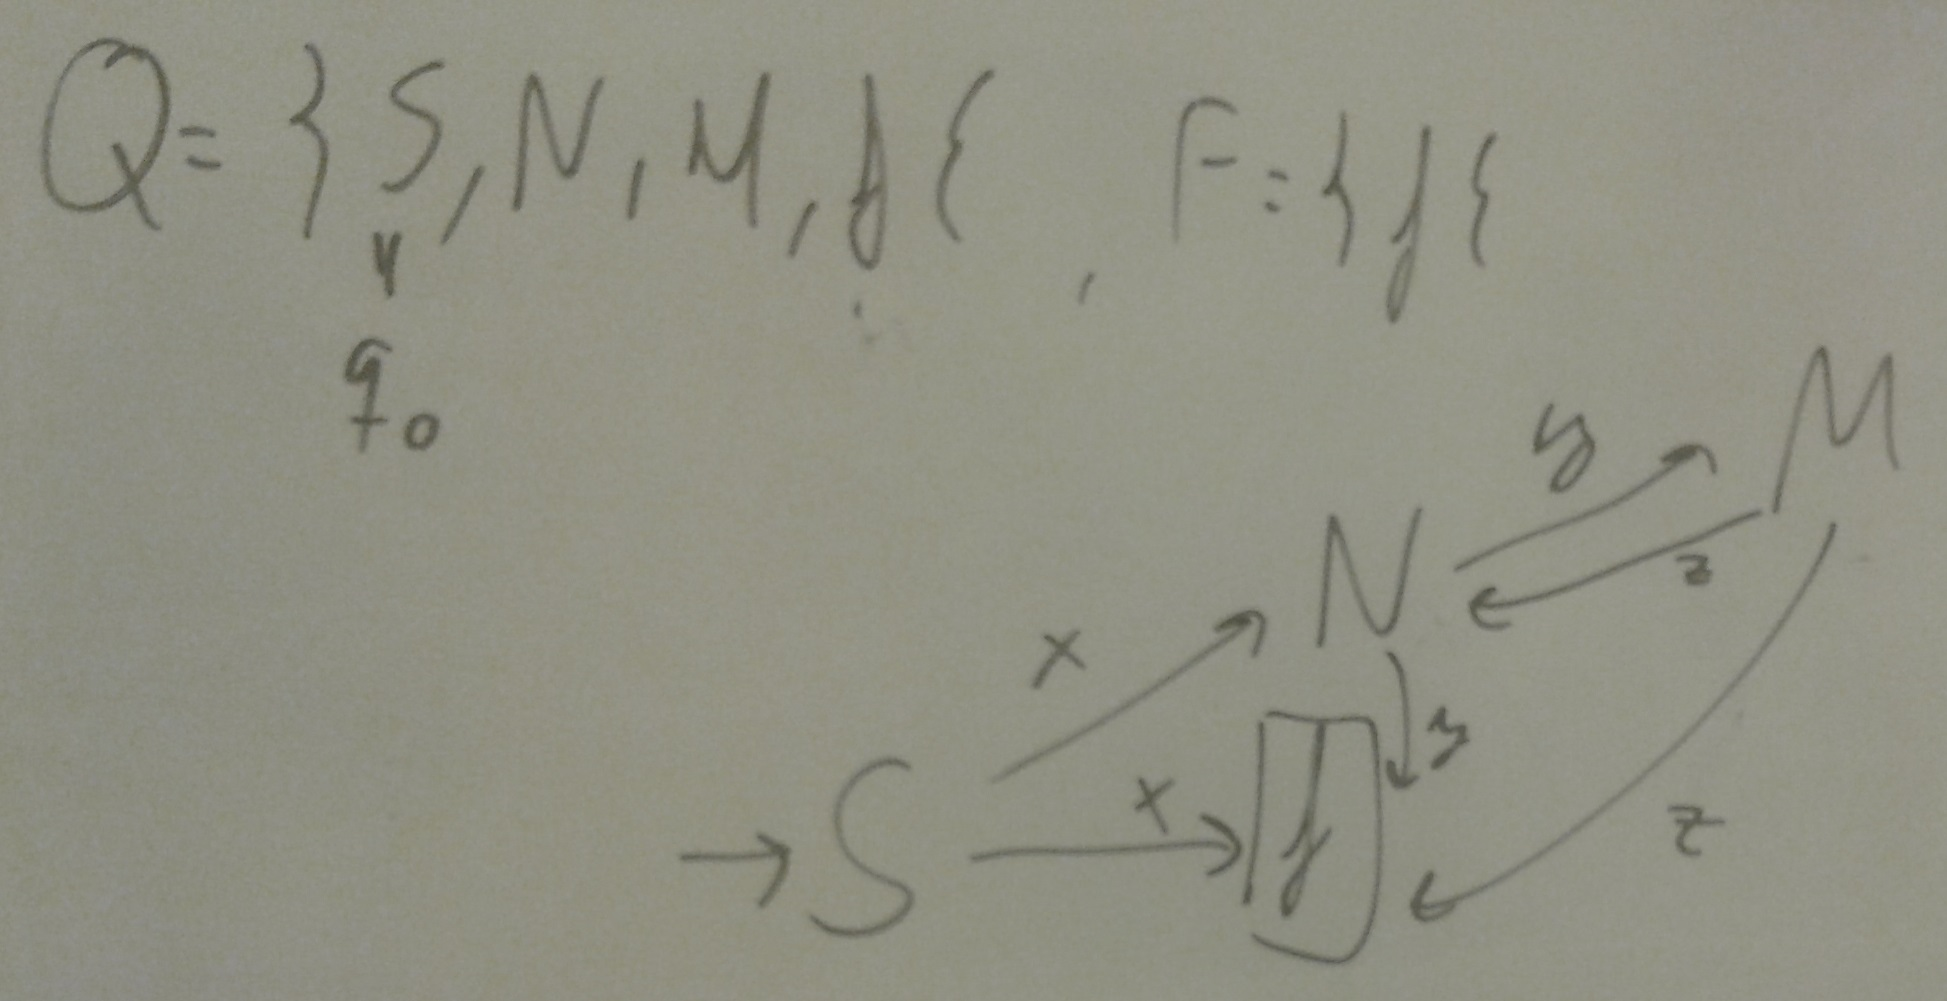
\includegraphics[scale=0.1]{Automatas/13-1}
\end{figure}
\begin{figure}[h!]
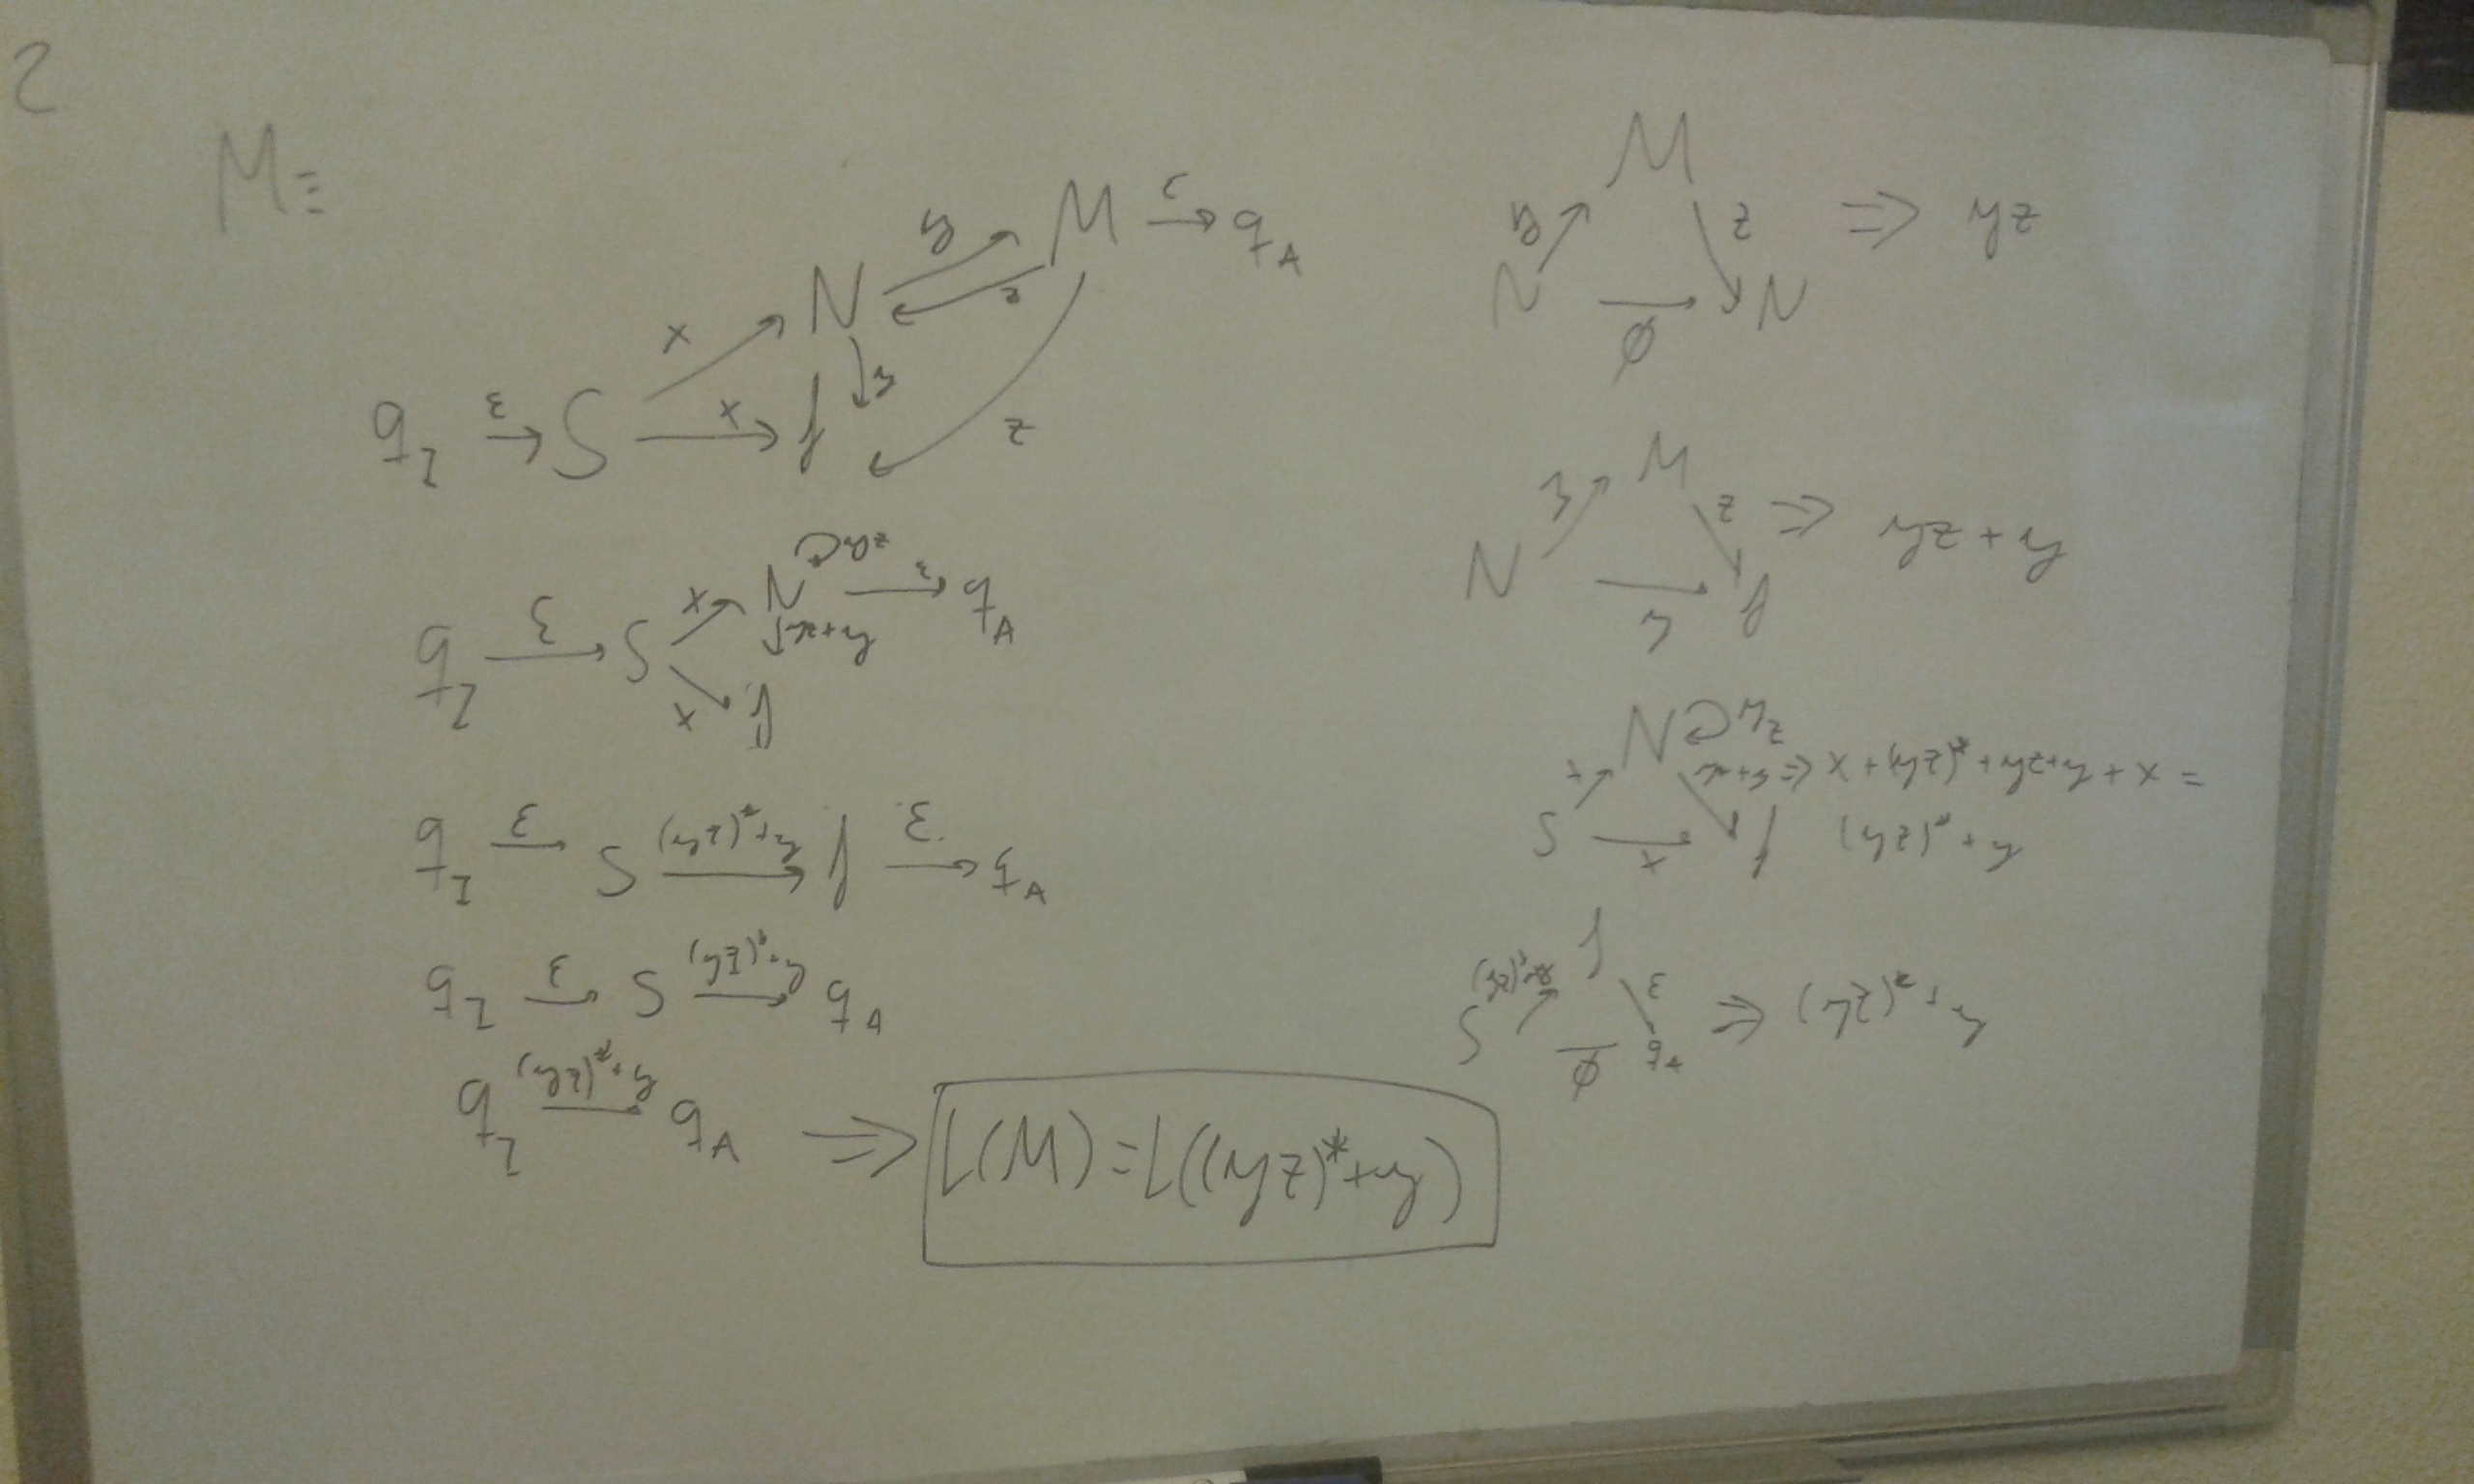
\includegraphics[scale=0.12]{Automatas/13-2}
\end{figure}\
\end{solucion}

\newpage

\begin{ejercicio}{14}
La siguiente gramática genera el lenguaje $\underline{0}^*\underline{1}(\underline{0} + \underline{1})^*$:
\begin{align*}
&S \rightarrow A1B\\
&A \rightarrow 0A\\
&A \rightarrow \varepsilon\\
&B \rightarrow \varepsilon\\
&B \rightarrow 0B\\
&B \rightarrow 1B\\
\end{align*}
siendo $\{S, A,B\}$ variables, $\{0, 1\}$ terminales y $S$ el símbolo inicial. Obtener derivaciones de las siguientes
palabras:
$$00101,\quad 1001,\quad 00011$$
\end{ejercicio}
\begin{solucion}
$$
S \rightarrow A1B \rightarrow 0A1B \rightarrow 00A1B \rightarrow 001B \rightarrow 0010B \rightarrow 00101B \rightarrow 00101
$$
$$
S \rightarrow A1B \rightarrow 1B\rightarrow 10B\rightarrow 100B\rightarrow 1001B\rightarrow 1001
$$
$$
S \rightarrow A1B \rightarrow 0A1B\rightarrow 00A1B\rightarrow 000A1B\rightarrow 0001B\rightarrow 00011B\rightarrow 00011
$$
\end{solucion}

\newpage

\begin{ejercicio}{15}
Sea $G$ la gramática regular que tiene como producciones:
$$\{S \rightarrow abA, S \rightarrow B, S \rightarrow baB, S \rightarrow \varepsilon, A \rightarrow bS, B \rightarrow aS, A \rightarrow b\}$$
siendo $S$ el símbolo inicial, $a, b$ terminales y $A,B$ variables. Construir un $\varepsilon$-AFND que acepte el
lenguaje generado por $G$.
\end{ejercicio}
\begin{solucion}
Desarrollemos un poco el árbol de derivación de $G$:
\[
\begin{tikzpicture}
  \node {S}
    child { node {abA} 
      child { node {abbS} } 
      child { node {abb} } }
    child { node {B} 
      child { node {aS} } }
    child { node {baB} 
      child { node {baaS} } }
    child { node {ϵ} };
\end{tikzpicture}
\]
Entonces $G$ genera el lenguage $(a+abb+baa)^*$. Construimos un $ϵ$-AFND que acepte este lenguaje:
\[
\begin{tikzpicture}[shorten >=1pt,node distance=2cm,on grid,auto] 
   \node[state,initial,accepting] (q_0)   {$q_0$}; 
   \node[state] (q_1) [above right=of q_0] {$q_1$};
   \node[state] (q_2) [below right=of q_0] {$q_2$};
   \node[state] (q_3) [right=of q_1] {$q_3$};
   \node[state] (q_4) [right=of q_2] {$q_4$};
    \path[->] 
    (q_0) edge node [below] {a} (q_1)
          edge node [below left] {b} (q_2)
    (q_1) edge [bend right] node [above] {ϵ} (q_0)
          edge node {b} (q_3)
    (q_3) edge node {b} (q_0)
    (q_2) edge node [below] {a} (q_4)
    (q_4) edge node [above] {a} (q_0);
\end{tikzpicture}
\]
\end{solucion}

\newpage

\begin{ejercicio}{16}
Describir una gramática regular que genere el lenguaje aceptado por el siguiente
autómata:
\end{ejercicio}
\begin{solucion}
\end{solucion}

INTENTAR HACER LOS DEL PUMPING LEMMA (17,18,19)
\end{document}